\documentclass[times,12pt]{ACME2015article}
\usepackage{amsmath,amssymb,amsthm,mathrsfs,graphicx}
\usepackage{subfigure}
\usepackage{titlesec}
\usepackage{algorithm}
\usepackage{algorithmic}
\usepackage{color}
\usepackage{float}
\usepackage{graphicx}
\usepackage{rotating}
\usepackage{url}
\usepackage{lastpage}
\usepackage{fancyhdr}

\pagenumbering{arabic}

\newenvironment{lyxcode}
{\par\begin{list}{}{
\setlength{\rightmargin}{\leftmargin}
\setlength{\listparindent}{0pt}% needed for AMS classes
\raggedright
\setlength{\itemsep}{0pt}
\setlength{\parsep}{0pt}
\normalfont\ttfamily}%
 \item[]}
{\end{list}}

\setlength{\parindent}{0pt}
\setlength{\parskip}{5pt plus 2pt minus 1 pt}

\topmargin  -25mm
\evensidemargin 0mm
\oddsidemargin  0mm
\textwidth  160mm
\textheight 267mm
\frenchspacing
\sloppy
\titlespacing{\section}{0pt}{\parskip}{0.01\parskip}
%%%%%%%%%%%%%%%%%%%%%%%%%%%%%%%%%%%%%%%%%%%%%%%%%%%%%%%%%%%%%%%%%%%%%%%
\begin {document}
\pagestyle{plain}

\begin{center}
{\fontsize{22}{20}\bf Calculating the Minimum Distance Between Pairs of Triangles on SIMD Hardware for DEM and Unstructured Mesh Contact Point Generation\\
}\end{center}

\vspace{\fill}
\begin{center}\fontsize{16}{20}
\textbf{Konstantinos Krestenitis$^1$}\\
01/06/2015
\end{center}
\vspace{\fill}

\begin{center}
{\fontsize{10}{12}
}\end{center}


\begin{center}
$^1$School of Engineering and Computing Sciences, University of Durham, DH1 3LE, Durham\\
konstantinos.krestenitis@durham.ac.uk\\
Mechanics Research Group\\
\end{center}
\begin{center}
Supervised by\\
Dr Tomasz Koziara\\
Dr Tobias Weinzierl\\
Professor Jon Trevelyan\\
\end{center}

\clearpage

\tableofcontents

\clearpage

\section{Introduction}
In contact mechanics and specifically in the discrete element method, it is an essential task to be able to calculate the distance between discrete elements. Distance calculation is used for surface and mesh generation if triangles are chosen as the primary element. Triangulated meshes are ideal for contact mechanics simulations because complex multi-facade shapes can be described by reducing the polyhedron shape to only triangles. Spherical objects are an exception because they are are best described as sphere elements instead of polyhedrons or triangles. Due to the fact that multi-facade objects can be reduced to triangular description individual triangle element can be computationally ideal to handle in the context of discrete element method both numerically but also computationally in parallel computational architectures. Calculating the distance between pairs of triangles in three dimensions will become an important task for contact simulations in the context of discrete elements method as it would be the state of the art approach for resolving contact detection using triangulated surfaces.

It is important to investigate the problem of finding the minimum distance between triangles because of the changes in the computational hardware [7]. The central processing unit architecture today and the future upcoming hardware [7] support Single Instruction Multiple Data (SIMD)[41] parallelism which allow on a singles core to be able to have data level parallelism, which theoretically can allow for four (double precision) and eight times (single precision) speedup. These speedups are enabled because of the wider vector widths and new instruction sets (SSE, AVX), which will widen more in the future [7]. In addition to single core speedups, processors are hosting multiple cores and in the case of high performance computing infrastructure that is usually involved in simulations there are multiple processors. It is vital to be able to extract all resources available on the current and future upcoming hardware, because the speedups enable more triangles to be used to describe triangulated bodies. Consequently enabling engineers to use an algorithm that is capable to handle the maximum amount of triangles per time step for the corresponding computational machinery. It would allow scientists to handle complex non-spherical objects (state-of-the-art today [27, 15]), to do better engineering and science.

Calculating the minimum distance between triangles can be categorized into two solving strategies; one is the naive or brute force approach where the geometric primitives of the triangles are compared. Geometric primitives of triangles include segments and points and the triangle plane. The alternative approach is to analytically describe the triangles based on their barymetric coordinates and then to create a nonlinear optimization problem based on the minimum distance relationship that describe the distance between them. Alternative iterative method is more favorable in terms of its computational complexity. Compared to the brute force method, it is less prone to data dependency, and due to its algorithmic nature, it is possible to avoid logical branching during computation. Avoiding logical branching is a key factor when writing vectorizable code for SIMD parallelism [32]. The iterative approach is found to be vectorizable and ideal for exploiting to the fullest the available CPU architecture. However the brute force approach is the robust method for calculating the minimum, it always yields correct results while iterative variants may not converge because of machine precision and the given regularization parameters.

The state-of-the-art work done in this area, to the best of my knowledge, doesn't involve studies on data parallelism at the level of triangle to triangle distance calculation nor any proposal for using analytic methods to this specific geometric triangles problem. In addition, in the context of discrete element method simulation, only the use of spheres in high performance computing environments is widely understood and implemented [15]. There is not much work on non-convex polygon meshes using non-spherical elements because of computational cost [27]. Additionally, algorithms that describe surfaces using watertight polyhedrons fail to perform contact point generation robustly [21]. Because contact point generators that rely on polyhedron shapes use variants of the GJK (Gilbert Johnson Kerthi) [3] algorithm that require the interpenetration of the shapes which causes contact divergence [26].

This report provides new insight into practical computational methods for the parallel computation of the brute force method. In addition it provides the introduction of the analytic approach as well as comparisons results of iterative solutions of the triangle-to-triangle minimum distance problem. The paper also provides insight into parallel implementation of the iterative method as well as comparable performance results using the GCC (GNU Compiler Collection) [23], Intel compilers in C++ programming language for SIMD (Single Instruction Multiple Data) [24], multicore processing (OpenMP)[37], and Intel ISPC  [23] for SIMD in C. This provides enough information for someone that want to use the algorithm and use it in practice in a discrete element method simulation package [15,28].

Besides applications-related studies the research investigates programming methodologies for optimized SIMD computation, and it goes through the process of optimizing sequential algorithms into optimized parallel variants. To achieve this, we distinguish two major strategies; evolutionary and revolutionary coding [7]. Both approaches have their own characteristic benefits and disadvantages in the process of development. The evolutionary approach parallelizes the code incrementally many times by trial and error and sequential enhancement of the implementation using compiler specific instructions. The revolutionary approach on the other hand rewrites the whole code using new language features to manipulate hardware directly, This approach gives the author the power for more control and the computational performance gain but also increases the risks for algorithmic bugs and decreased the maintainability of the code in favor of performance. In the context of computing the distance between pairs of triangles, both evolutionary and revolutionary parallization approaches using brute force and iterative methods show significant computational speedups from their original counterparts. In this investigation, it is found that a mix of revolutionary firstly and then evolutionary enhancements using code with compiler specific instructions is the optimal technique to achieve the best performance results.

The remainder of the paper is structured as follows. In Section 2, the popular method of using the GJK [3] algorithm is reviewed that only works for watertight polygon shapes that cannot be computationally efficient as well as robust due to penetration. The enhanced meshing method 'boundary layer triangular meshes' [21] for improved contact detection and robustness thus is reviewed; Next, in Section 4, the brute force method is analyzed as well as its major computing components. In Section 5, the iterative method is investigated as well as a detailed comparison study between different approaches. In Section 7, the implementation of the brute force method as well as the fastest iterative method is introduced as in serial and parallel variants and all the rigorous implementation techniques for the underlying hardware are described. In Section 7, a detailed performance study is given. Section 8, discusses the future research plans.


\section{Contact Point Generation}

Two ways of detecting contact between two bodies is using convex shape description, and description of only the surface of two bodies. The first case (Section 2.1), the GJK algorithm[12]; convex shape contact detection requires that the bodies simulated to be described using polyhedron elements. And because contact detection in GJK involve the necessary allowance of convex shapes penetrating each other, it creates the problem of contact divergence (Figure \ref{fig1}).

\begin{figure}[!h]
\centering

\includegraphics[width=0.3\textwidth]{divergence} \protect\caption{\label{fig1}Contact divergence situation due to penetration. Where A,B are convex bodies, x1,x2 contact points with normals, d1,d2 is the penetration depth. In the next time step object A will move upwards to the right and object B downwards to the left.}
\end{figure} 

To understand the problem of divergence 2D shapes; (Figure \ref{fig1}) The minimum penetration depths d1,d2 from the two bodies A,B give rise to one vertical and one horizontal contact. When simulated, this contact formation will lead to a rightward rotation for object A, which would cause increased penetration on the next timestep, thus creating an unpredictable outcome during the simulation. This problem is found in simulation software that uses GJK algorithms variants[27]. 

To overcome the problem of divergence, leads us to the second method for detecting contact between two bodies (Section 2.2). In this approach interpenetration is avoided by introducing a boundary layer around the bodies. This method involve description of the surface of the bodies using non-convex triangles in 3D. Leading to motivate the research in calculating the distance between pairs of triangles. The two approaches are reviewed as part of the literature review, and they acts as the reason behind this research which involve triangles in context of contact detection.

\subsection{The Gilbert Johnson Keerthi Distance Algorithm}
The GJK algorithm [3, 12, 13] is one way for contact detection. The algorithm operates on convex bodies only, and can only provide collision detection where there is penetration. Non-convex bodies cannot work using GJK, making contact detection for triangles in 3D space impossible. The following section is a literature review and shows how GJK is used, for the purpose of understanding that this variant of algorithms introduce problems in simulations due to body penetration (contact divergence).

The algorithm relies on the Minkowski Sum operation. For two shapes, the Minkowski Sum of those shapes is all the points in shape1 added to all the points in shape2: $A + B = {a + b \:|\: a \in A, \: b \in B}$. If both shapes are convex, the resulting shape is convex. The significance is not in the addition but in the subtraction $A - B = {a - b. \:\:|\:\: a \in A, \: b \in B.}$ because if two shapes are intersecting the Minkowski Difference will contain the origin.

\begin{figure}[!h]
\centering
\includegraphics[width=1\textwidth]{gjkshapes} \protect\caption{\label{fig2}left: Two convex shapes intersected. right: Minkowski Difference of the two shapes.}
\end{figure} 

Performing the Minkowski Difference on the two shapes in Figure \ref{fig2}, left yield the shape in Figure \ref{fig2}, right where the shape contains the origin. The enclosure of the origin indicate that the two shapes are in contact or intersection. Performing the Minkowski sum requires subtractions along the vertices but it is sufficient to perform the subtraction on selected vertices instead of computing the whole Minkowski difference. As long as it is possible to ensure enclosure or disclosure of the origin within the Minkowski Difference, the algorithm can determine whether or not the shapes are in contact. Executing the GJK algorithm iteratively, a polygon is build within the Minkowski Difference.

In order to build the simplex polygon a support function is used. The support function returns a point in the Minkowski Difference given two shapes. Take a point from shape1 and shape2, take their difference, and obtain a corresponding point in the Minkowski Difference and progressively build the polygon. To enhance this process of constructing the polygon, a right origin direction is needed so that the simplex is build around the origin faster, to subsequently indicate that Minkowski Difference enclose it or not. 

It is significant to take the farthest point towards a direction at each iteration using the support function because the simplex creation should contain a maximum area therefore increase the chance that the algorithm converge quickly (Algorithm \ref{alg1}). Because of that, all the points returned by the support function should lie on the edge of the Minkowski Difference, therefore any point past the origin along some direction, cannot contain the origin. Using the shapes in Figure \ref{fig2}, left and performing the support function three times, the points of the new simplex results to a triangle:

\begin{algorithm}
\begin{lyxcode}
1.~~[point] = \textbf{\textcolor{blue}{support}}(shape1, shape2, Vector d) 

2.~~~~p1 = shape1.FarthestPointInDirection(d)

3.~~~~p2 = shape2.FarthestPointInDirection(-d)

4.~~~~\textbf{\textcolor{blue}{return}} (p1 -  p2)

\end{lyxcode}
\protect\caption{\label{alg1}Pseudocode Support Function}
\end{algorithm}

The best-case scenario is when only a triangle is created (three iterations, three simplex points) and we conclude whether there is an intersection or contact between the two convex shapes if the new shape includes the origin.

  \begin{figure}[!h]
\centering
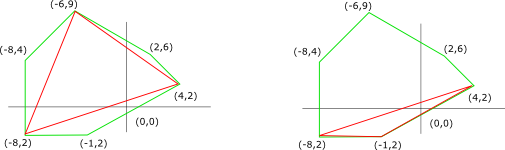
\includegraphics[width=0.8\textwidth]{2} \protect\caption{\label{fig3}left: Simplex where origin is not enclosed right: Simplex including origin}
\end{figure} 

To detect collision, the direction of search towards origin is the key factor in the iterative process. If the third point in the simplex does not contain the origin, the algorithm has to recalculate another point and use that instead. It is not possible to guarantee that the first formed triangle can contain the origin nor it is guaranteed that the Minkowski Difference contains the origin, that's the the case where there is no contact. It is only possible to modify how the individual points are chosen based on a direction towards the origin.

\begin{algorithm}
\begin{lyxcode}

1.~~d = initial guess

2.~~a = \textbf{\textcolor{blue}{support}}(d) 

3.~~b = \textbf{\textcolor{blue}{support}}(-d)

4.~~AB = b - a

5.~~AO = ORIGIN - a

6.~~d = (AB x AO) x AB

7.~~c = \textbf{\textcolor{blue}{support}}(d)
\end{lyxcode}
\protect\caption{\label{alg2}Pseudocode for direction towards origin}
\end{algorithm}

The process of iteration starts as follows; (See Algorithm \ref{alg2}) initial guess for a first direction d is provided (line 1) , then progressively the simplex is created but such iterations are kept low and in a direction that contain the origin so convergence is fast (line 4-6). 

There are two conditions for convergence:
\begin{enumerate}
\item Simplex is containing the origin 
\item There is a direction d that enclose origin by modifying the simplex.
\end{enumerate}

\begin{algorithm}
\begin{lyxcode}

1.~~ d = initial guess 

2.~~simplex.add(support(d)) 

3.~~\textbf{\textcolor{blue}{WHILE}} (1)

4.~~~~simplex.add(support(d));

5.~~~~\textbf{\textcolor{blue}{IF}}  dot(simplex.getLastPoint, d) <= 0 

6.~~~~~~\textbf{\textcolor{blue}{return}} false 

7.~~~~\textbf{\textcolor{blue}{ELSE}}  

8.~~~~~~\textbf{\textcolor{blue}{IF}} simplex.containsOrigin 

9.~~~~~~~~\textbf{\textcolor{blue}{return}} true 

10.~~~~~\textbf{\textcolor{blue}{ELSE}} 


11.~~~~~~~d = newDirection(Simplex) 

12.~~~~~\textbf{\textcolor{blue}{ENDIF}} 

13.~~~\textbf{\textcolor{blue}{ENDIF}} 

14.~~\textbf{\textcolor{blue}{ENDWHILE}}
\end{lyxcode}
\protect\caption{\label{alg3}Pseudocode of iterative GJK algorithm.}
\end{algorithm}
 
\begin{figure}[!h]
\centering
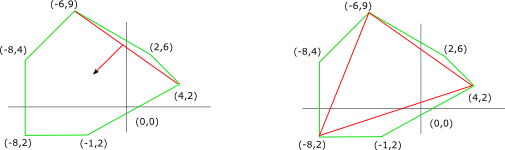
\includegraphics[width=0.8\textwidth]{3} \protect\caption{\label{fig4}left: First iteration. right: Second iteration}
\end{figure} 

\begin{figure}[!h]
\centering
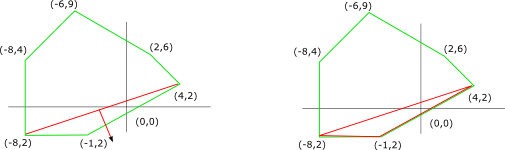
\includegraphics[width=0.8\textwidth]{4} \protect\caption{\label{fig5}left: Backtrack iteration, set simplex, direction. right: Third iteration; determined contact. }
\end{figure}

To enhance the iterative process, a search for a direction that contain origin is performed by a series of plane checks. If the line segment is defined as A to B where A is the last point added to the simplex. Both A and B are on the edge of Minkowski Difference and the origin cannot lie in either normal direction (See Algorithm \ref{alg3}). The origin can only lie in the rest uncovered area. And because a line segment cannot contain the origin, a third point is required to be found. Using the perpendicular of AB in the direction of origin: perp = ((B-A) x (O-A)) x (B-A) (line 6 - Algorithm \ref{alg2}), if the origin O lies on the segment then the perpendicular will be a zero vector. This happens in two places:
\begin{enumerate}
\item inside the Minkowski Sum 
\item on the edge of the Minkowski Sum.
\end{enumerate} 
The second iteration turns the simplex into a triangle. The regions do not have to be tested since the origin cannot be at any of those points since each point is added because they passed the check in the algorithm. We can perform (AC x AB) x AB to yield the perpendicular vector to AB. By performing dot(Perpendicular(AB), AO) it is possible to determine whether the origin is in region. 

The GJK algorithm for contact point generation is not favorable for particle simulation as it is only working for convex polyhedrons that allow penetration. Contact detection using GJK requires allowance for penetration which result in contact normal divergence problems (See Section 2.2 for contact divergence). Contact divergence can be mitigated, but by adding checking mechanisms in place (contact clustering) [26] and these result in additional computational overhead in the simulation.


\subsection{Boundary Layer Expanded Meshes}
The other method to calculate the distance between triangulated bodies is using unstructured meshes. The idea of using unstructured meshes for contact detection is developed in the area of robotics simulation [22]. In this concept[21], it is introduced a robust contact generation technique where the boundaries of the bodies are fattened with a margin to provide stability, especially useful for meshes that include features with noise. 

To overcome divergence (as discussed in Section 2. introduction) there must be a restriction to the penetration depth when in contact. The current method applies a approach to rigid-body meshes, with the primary effect of producing stable contact estimates for mesh-mesh collisions and tolerating numerical errors. The method consists of a triangle mesh M along a margin width parameter $r \geq 0$, and treats collisions with the Minkowski sum of M and a sphere $B$ at the origin with r being the radius: $G=M \oplus B(0,r)$
The contact between object A and B, represented as $(MA, rA)$ and $(MB,rB)$, is to occur when $(MA \: xor \: B(0,rA)) \cap (MB \: xor \: B(0,rB)) \neq 0$ .

\begin{figure}[!h]
\centering
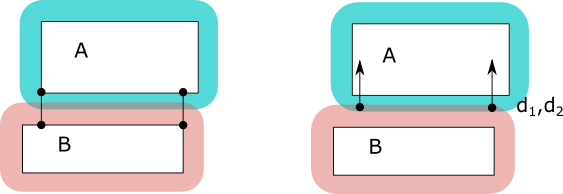
\includegraphics[width=0.6\textwidth]{contact1} \protect\caption{\label{fig6}Contact divergence is avoided by introducing boundary layers in the two bodies, prohibiting penetration making contact point generation robust. Left figure show contact points on A,B. Right figure show contact normal caused by contact. d1,d1 is the boundary margin penetration depth. See Figure 1 for contact divergence example when penetration is allowed.}
\end{figure} 

The boundary layer approach computes plausible contact points from the closest points on nearby triangles on the underlying meshes MA and MB. In addition to detecting collision, contact points, normal, and penetration depths are resolved so that an instantaneous motion of each point on object A in the direction of the normal reduces penetration depth.

For example, for a set of n triangles $t_i$ in a mesh M, the Minkowski sum of M and a sphere is the union of the fattened triangles: $M \: xor \: B(0, r) = t_i \:xor\: B(0, r)$. The bodies $(MA, rA)$ and $(MB, rB)$ are in contact if for a pair of triangles $t_i$ in $MA$ and $t_j$ in $MB$: 
$$(t_i \:xor\: B(0,rA +rB)) \cap t_j \: \neq 0.$$
This can be used in a function $d(t_i,t_j)$ that computes the exact minimum distance between triangles $d(t_i,t_j) \leq rA+rB$.

The contact generator outputs a single contact point for all pairwise triangles within distance $rA +rB$. The penetration depth is:
$$p = rA + rB - ||xA - xB||. $$

The contact normal is: 
$$n = (xA - xB) / (||xA - xB||).$$ 

The contact point is: 
$$(xA + xB)/2 + n \times (rB-rA)/2$$

and is placed in the middle of the overlap region. If the triangles intersect, then shortest retraction among all candidates as illustrated in Figure \ref{fig7} is the contact point on the body. However, once triangles penetrate, the simulator loses robustness. That is because of the undefined contact point, that can no longer be defined due to the penetration (contact divergence), making impossible the passing of the required contact normal information to the next time step of the simulation. 

\begin{figure}[!h]
\centering
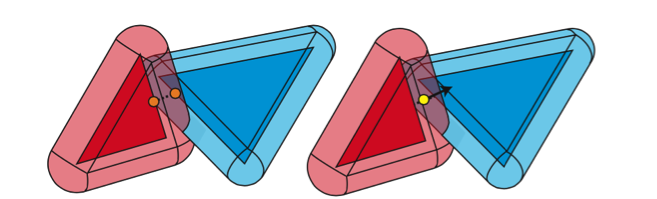
\includegraphics[width=0.8\textwidth]{contact2} \protect\caption{\label{fig7}Contact points (left) and contact normal (right) using boundary margin layer triangles for contact generation robustness.[21]}
\end{figure} 

The closest points on the triangles correspond to the deepest penetrating points of the expanded triangles. The triangles are in contact when for all pairs of triangles there is a pair whose distances are less than the sum of the extended margin. This can also be expressed using the minimum distance between triangles.

\begin{figure}[!h]
\centering

\includegraphics[width=1\textwidth]{contact3} \protect\caption{\label{fig8}Example of triangles that intersect without boundary layers; the direction of shortest retraction is not consistent. This make the contact point generation not robust, causing contact divergence. As it can be seen in the right figure where the black arrow indicate how the triangle should move in the next time step, making the kinematics of the simulation inconsistent.[21]}
\end{figure} 

\clearpage

\section{Triangle Distance Problem}
The problem of constructing the fastest method for generation of the contact points is reduced to calculating the minimum distance between pairs of triangles in 3D. To my knowledge there is only one strategy to obtaining the distance between two triangles robustly. The known method is by brute force. It checks the distances of the triangles primitives, vertices and segments. The brute force method to my knowledge is only found in sequential codes, i introduce an optimal vectorizable version of and a study of its computational components. In this report, we further introduce alternative iterative methods, using nonlinear optimization for calculating the minimum distance. The objective is to find an optimal algorithm that is suitable for SIMD (Single Instruction Multiple Data) processing hardware[41, 24] robust. 

\section{Brute Force Approach}
The brute force or naive approach, calculates all the distances between geometrical primitives of the triangles. These calculations include checking the distance between every segment of one triangle (segment – segment distance) with the other, and every  point one triangle to the other triangle [8,9,10]. This requires checking of the minimum distance among all comparisons in order to find the overall minimum distance. Let $v_{1i}$, $e_{1i}$, $v_{2i}$, $e_{2i}$ be the vertices and edges of triangles $T_1$ and $T_2$. The brute force approach computes all fifteen distances $v_{1i}$-to-$T_2$, $v_{2i}$-to-$T_1$, $e_{1i}$-to-$e_{2i}$, and then selects the smallest. This approach is quite simple to implement. Optimization of this method can at most rely on reusing parts of the computation, but it is not possible to avoid a relatively complex branching because of its nature that requires a number of if statements. Therefore it is difficult to optimize this approach for SIMD parallelism.

\begin{algorithm}
\begin{lyxcode}
\textbf{\textcolor{blue}{function}}~minDistance~=~\textbf{BruteForce solver}(T1, T2)

1~~\textbf{\textcolor{blue}{FOR}}~i=1:9

2~~~~$seg_{i} =segseg(segT1_{i}, segT2_{i})$

3~~\textbf{\textcolor{blue}{ENDFOR}}

4~~$minSegDistance = min(seg_{i})$

5~~\textbf{\textcolor{blue}{FOR}}~i=1:3

6~~~~$pt_{i} = pointTriangle(p_iT1, T2)$

7~~~~$pt_{i+3} = pointTriangle(p_iT2, T1)$

8~~\textbf{\textcolor{blue}{ENDFOR}}

9~~$minPointTriangleDistance = min(pt_{i})$

10~~*minDistance = min(minSegDistance, minPointTriangleDistance)

\end{lyxcode}
\protect\caption{\label{alg4}Brute Force TTD Pseudocode.}
\end{algorithm}


\subsection{Segment to Segment Minimum Distance }
The calculation of the distance between segments [8,9] in three dimensions is a geometric calculation that involve getting the closest points by the extending the line that they lie on until intersection, if the two lines intersect then the closest point on the two segments is on the boundaries of the segment.
The segment 
$$S1 = [P0, P1]$$
can be formulated as 
$$P(s) = P0+s(P1-P0) = P0+su$$
with a constraint on s, $0<=s<=1$. Similarly, the second segment 
$$S2 = [Q0, Q1]$$
is written as $$Q(t) = Q0+t(Q1-Q0) = Q0+tu$$ with constraint $0<=t<=1$. So, for $sC$ and $tC$ being the closest points on the corresponding extended segments lines L1 and L2, then if  both sC and tC are within the boundaries of the segments then the closest points are also the closest points on the respective segments. 
In the case where sC and tC correspond to points on L1 and L2 outside the range of either segment $S1$ and $S2$, then sC and tC do not also define the closest points on the segments $S1$ and $S2$. So it is necessary to determine points that minimize 
\begin{equation}
w(s,t) = P(s) - Q(t)
\end{equation}
over the ranges of the segments using the corresponding constraints. 
The problem can be formulated into a minimization problem where the equation w is the same as minimizing 
$$|w|^2 = w \cdot w= (P0+su-tv) \cdot (Q0+su-tv)$$

which is a quadratic function of s and t. The relation of $|w|^2$ define a parabolic equation over a (s,t)-plane (See Figure \ref{fig9}) with a minimum at $C = (sC, tC)$, it is strictly growing along the (s,t)-plane with starting point from C. But because segments $S1$ and $S2$ are concerned and not their respective extended lines $L1$ and $L2$, the required minimum region is not C but it is located over a subregion G of the (s,t)-plane. The global minimum at C may lie outside of G, however, in these cases, the minimum always occurs on the boundary of G, and in particular, on the part of G's boundary that is visible to C. That is, there is a line from C to the boundary point which is exterior to G, and it can be said that C can "see" points on this visible boundary of G (See Figure \ref{fig9}).

\begin{figure}[!h]
\centering

\includegraphics[width=0.3\textwidth]{ss_box} \protect\caption{\label{fig9}(s,t) parameter space with G boundary box C for global minimum}
\end{figure} 

Suppose that we want the minimum distance between two finite segments $S1$ and $S2$, then 
$$G=\{ (s,t) \: \| \: 0 \leq s \leq 1, 0 \leq t \leq 1 \} = [0,1]\times[0,1]$$ 
is a unit square in (s,t) space. The four edges of the square are given by point at $s = 0, s = 1, t = 0, t = 1$. If $C = (sC, tC)$ is outside the G area, then it can "see" at most two edges of G. If $sC < 0$, C can see the $s = 0$ edge, if $sC > 1$, C can see the s = 1 edge, and similarly for tC, so in this way there is an enforcement of the required constraints. When C is not in G, at minimum 1 and at maximum 2 of constraints are active, and they determine which edges of G are candidates for a minimum of $|w| ^2$.
 
For each candidate edge, to compute where the minimum that occurs on that edge, either in its interior or at an endpoint, it is possible to solve for the other unknown parameter since at minimum one is to be found (either t or s). So using the derivative of the $|w^2|$ equation it is always possible to solve for the parameter that is in the interior of G. For example when s = 0, $|w|^2 = ((P0-Q0)-tv) \cdot ((P0-Q0)-tv)$. Taking the derivative with $t$ it possible get a minimum when: $0 = \frac{d}{dt}|w|^2 = -2v \cdot ((P0-Q0)-tv)$.
This gives a minimum on an edge at (0, t0) where $t0 = \frac{(v \cdot (P0-Q0))}{(v \cdot v)}$
If $0 <= t0 < 1$, then this would be the minimum of $|w|^2$ on G, and P(0) and Q(t0) are the two closest points of the two segments. But in the case where t0 is outside G, then either (0,0) or (0,1), would be the minimum along that edge (since $s=0$). Using this method it is possible to perform only a couple of checks to find the minimum of w(s,t) that correspond to the minimum distance between the segments.

\subsection{Point to Triangle Minimum Distance}
The other calculation required by the naive approach is to perform the check of point to triangle distance[12, 10, 11]. This test complete the brute force approach since it doesn't leave any  space for cases where triangles are in a configuration where a point - triangle plane distance is the shortest distance in the initial triangle pair minimum distance problem. 

To understand the problem of computing the minimum distance between a point P and a triangle T, it is necessary to understand the parameterized coordinate system of triangles. A triangle can be described by its barycentric coordinates in a way that any point on it can be dependent on two parameters, such that 

$$T(s, t) = B + s \cdot E0 + t \cdot E1$$

where $B = point1$, $E0 = point2-point1$, $E1 = P3 - P1$ for 

$$(s,t) \in D = \{(s,t) : s \in [0,1],t \in [0,1],s + t ≤ 1\}$$ 

The minimum distance is computed by determining the values $(s, t) \in D$ in the squared-distance equation $Q(s, t) = |T(s, t) - P|^2$ where $T(s,t)$ correspond to a point on the triangle closest to P. The function is quadratic and can be written as: 
$$Q(s,t)=as^2 +2bst+ct^2 +2ds+2et+f$$

where $a = E0 \cdot E0$, $b = E0 \cdot E1$, $c = E1 \cdot E1$, $d = E0 \cdot (B - P)$, $e = E1 \cdot (B - P)$, and $f = (B - P) \cdot (B - P)$.

Quadratics are classified by the sign of $ac - b^2$ so for function Q, $ac - b2$ = $(E0 \cdot E0)(E1 \cdot E1) - (E0 \cdot E1)^2$ =$|E0 \cdot E1|^2 >0$. The positivity is based on the assumption that the two edges E0, E1 are linearly independent, so their cross product is a nonzero vector. Q is a continuously differentiable and the minimum occurs at an interior point of D where the gradient $Q = 2(as + bt + d, bs + ct + e) = (0, 0)$ or at a point on the boundary of D. The gradient of Q is zero only when 
$$s = (be - cd)/(ac - b^2)$$ and 
$$t = (bd - ae)/(ac - b^2).$$ 
If $(s,t) \in D$, then minimum of Q is found. For example considering that region 0 (See Figure \ref{fig10}) is the domain of Q, so $(s, t) \in D$. If (s, t) is in region 0, then the point on the triangle closest to P is interior to the triangle, not on its edge.

\begin{figure}[!h]
\centering
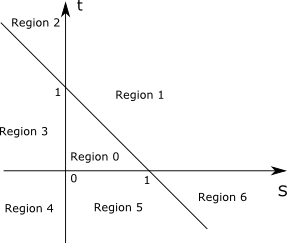
\includegraphics[width=0.4\textwidth]{pt_regions} \protect\caption{\label{fig10} Regions based on the (s,t) parameters plane}
\end{figure} 

On the other hand if the minimum is not in D then it should be should be on the boundary of the triangle and using the correct active constraints to restrict the solution using the region methodology. So if (s, t) is in region one then the elliptic level curves of Q are those curves in the s,t plane for which Q is constant. 

At the point where Q = (0,0), the level curve degenerates to a single point (s, t). The global minimum of Q occurs there ($V_{min}$). As the level values V increase from $V_{min}$, the corresponding levels are growing away from $(s,t)$. There is a smallest level value V0 for which the corresponding ellipse is tangent to the triangle domain $D$ edge $s+t = 1$ at a value $s = s0 \in [0,1], \: t0 = 1 - s0$. So for any level values $V < V0$, the corresponding ellipses do not intersect $D$. However for any portion of $D$ that intersect elliptic levels V must be $V > V0$. Therefore in this case point $(s0, t0)$ provides the minimum distance between P and the triangle where $t0$ is known $t0 = 1 - s0$ and $s0$ is the only unknown to be solved since the problem is decreased by one dimension. Moreover, when minimization is happening at $\nabla Q(s, 1 − s) = 0$ then there are three cases where $s > 1$ and $s$ has to be restricted to $s=1$ and the minimum occurs at $\nabla Q(1, 0)$ because of the barymetric triangle constraints, similarly if $s < 0$ then minimum occurs when $\nabla Q(0,1)$ or lastly $s \in [0,1]$ and has to be solved for a minimum at $\nabla Q(s,1-s)$.

Similarly the same technique for determining whether the minimum occurs at the endpoints or at the interior interval of the corresponding constraints, is performed for region three and region five (Figure \ref{fig10}). In the case where (s, t) occur in region three then the minimum has to occur at (0, t0) following the process like in region one where $t0 \in [0, 1]$. If $(s, t)$ is located in region five (Figure \ref{fig10}), then the minimum occurs at $(s0, 0)$ where $s0 \in [0, 1]$.  

When $(s, t)$ is located inside region two, there are three possibilities for the elliptic level curve that contact or intersect the boundaries of $D - region0$ area, the contact of the levels with the triangular region may occur in: 
\begin{enumerate}
\item edge where $s + t = 1$ 
\item edge where $s = 0$
\item at point where $t = 0$ and $s = 1$.
\end{enumerate}

That is because although the global minimum occurs in region two, there is a level curve of Q that contact the $D$ but the contact point and the region inside the level curve does not overlap. At these occurrences then the negative of the contacting level curve of Q cannot point inside $D$. For example for region two could be the direction of $-\nabla Q(0,1), -\nabla Q(s,1-t) and -\nabla Q(0,t),$ which points towards the inside of the level curve instead of inside $D$. 

In order to determine which of the three cases occur, it is possible to check which areas are negative so in a way it is possible to eliminate the cases where the contact doesn't occur and where it does. So if $\nabla Q = (Qs, Qt)$ and $Qs$ and $Qt$ are the partial derivatives of Q, it should be the case where $(0, -1) \cdot \nabla Q(0, 1)$ and $(1, -1) \cdot \nabla Q(0, 1)$ are not both  negative. The two vectors $(0, −1)$ and $(1, −1)$ are directions that correspond to the edges $s = 0$ and $s + t = 1$, respectively. The choice of edge $s+t = 1$ or $s = 0$ can be made based on the signs of $(0,-1) \cdot \nabla Q(0,1)$ and $(1, -1) \cdot \nabla Q(0, 1)$. Similarly as for region three, the same calculation technique is used for the regions four and six. 

\clearpage

\section{Iterative Approach}
The second approach to solving the triangle to triangle minimum distance problem is by parameterization of the triangles so that distance between them is formulated into a quadratic function and a minimization problem. This approach to the problem is iterative compared to brute force which is just getting the minimum value for all checks performed. The methods discussed are iterative because they approximate the solution using Newton method. That also characterizes the iterative approach as less naive since unnecessary geometric distance checks are not required to be performed.

The best iterative method calculates the minimum distance as a minimization problem but at the same time it has be to guaranteed that it is exploiting the SIMD type of CPU[24,41,39] architecture to yield the maximum computational capability of a modern processing unit instruction set. A numerical approach to the triangle to triangle distance problem is to form a nonlinear problem, that is possible to solve the minimum distance of the two triangles. It is possible to achieve this by parameterizing the triangles so that a nonlinear relation can be formulated. Every point on a triangle can be described as a function using their barycentric coordinates.

The optimized methods rely on an optimization based reformulation of the minimum distance problem. Triangles can be parameterized using barycentric coordinates[36]. Let $x$ and $y$ be two points, belonging respectively to triangle $T_1$ and $T_2$. Assuming that points $A, B, C$ are vertices of $T_1$ and that points $D, E, F$ are vertices of $T_2$, $x$ and $y$ can be defined using the following equations: 
\begin{equation}
T_{1}:x(a,b)=A+(B-A) \cdot a+(C-A)\cdot b
\end{equation}
\begin{equation}
T_{2}:y(g,d)=D+(E-D) \cdot g+(F-D) \cdot d
\end{equation} 
To find the minimum distance between $T_1$ and $T_2$ and the corresponding two closest points $P$, $Q$on the two triangles we minimize
\begin{equation}
f\left(a,b,c,d\right)=\left\Vert x\left(a,b\right)-y\left(c,d\right)\right\Vert ^{2}
\end{equation} 

What has to be noted is that for $x$ and $y$ to stay within the area of definition of the two triangles. The four parameters of the function $f$ have to comply with the six inequality constraints, requiring to find:
\begin{equation}
f(a,b,g,d)_{min}
\end{equation}  
$$such \:that: \: \{a\geq0,b\geq0, a+b\leq1, d\geq0, g\geq0, g+d\leq1 \}$$ 
This forms the basis of the optimization problem to be solved[14, 16].

\begin{figure}[!h]
\centering
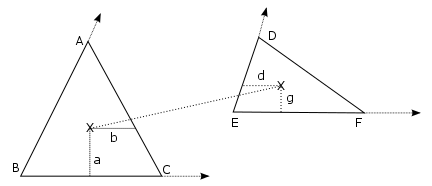
\includegraphics[width=0.5\textwidth]{c} \protect\caption{\label{fig11}Example of minimum distance and the corresponding barycentric points (parameters of objective function) on a pair of triangles in 3D. Triangle X:T1 has points A, B, C where barymetric parameters a,b correspond to point $x$ on the triangle. Triangle Y:T2 has points D,E,F where barymetric parameters g,d correspond to a point $x$. The two defined barymetric points define the minimum distance between the two triangles in 3D.}
\end{figure} 

For the optimization there are a couple of methods. The investigation had to go into efficient algorithm that take into account the ability to perform the minimization using vector processing. For searching the minimum of the parabolic geometry of the problem the Newton method is
 used [1,43]. Newton method involve using information from the curvature of the problem using the hessian and gradients [43] to arrive to a point that is the minimum. The steps to arrive to the solution are discrete and take into the constrained applied to the objective function. The minimization problem has to take into account the required constraints which forbid the closest points to be located outside the interval area of their corresponding triangles. To enforce the constraints, the constraint minimization has to be transformed into a series of unconstrained problems with the augmentation of the objective function $f$ with a constraint optimization method. An investigation began to pick up the best solver to be implemented for SIMD hardware. Floating-point operations and Newton steps were criteria to select the most suitable method. 

\subsection{Barrier Method}
During the exploration for suitable optimization approaches, a complete investigation would be lacking if it didn't include the testing of the barrier method [36,43] for enforcing the constraints, so it had to be incorporated into the series of tests for computational performance. The barrier method exploits a logarithmic function in order to incorporate the constraints into an extended objective function: 
\begin{equation}
B(x)=f(x)+r\sum_{i=1...6}-log(c(x_{i}))
\end{equation} cf. barrier figure, where r is the barrier parameter. The barrier method is characterized by its requirement to arrive at the solution from within the feasible region [36,43] ($B(x)$ is not defined outside of the feasible region).

\begin{figure}[!h]
\centering
\includegraphics[width=0.7\textwidth]{barrier} \protect\caption{\label{fig12}Illustration of a 2D problem where the logarithmic barrier function (red line) is added to the objective function (black line) f(x) to define feasible region (red line) under the constraint $a$ (dash line). }
\end{figure} 

The barrier method is characterized by its property to arrive to the solution from within the feasible region. It is known [136] that there are cases that the use of barrier method is not preferred because it is not always possible to have a initial guess value that is within the feasible region. But in the case of the the triangle to triangle distance problem that is not the case and an ideal initial guess values for the Newton method to start, are the barycentric center of the triangles. The method is prototyped on MATLAB for testing, and then ported for SIMD (Single Instruction Multiple Data) hardware using the Intel ISPC compiler [39].
 
In practice the use of Barrier method for solving constrained problems faces several computational difficulties[36,43]. That is due to the structure of the logarithmic barrier function and for the small values of the barrier parameter r, the search is facing ill-conditioning effects and round-off errors [36,43] when the search is approaching the boundary of the feasible region, the logarithmic function becomes infinite. As the boundary of the feasible region is approached and because the search is in discrete Newton steps, a step may lead to a region outside the feasible region. So an explicitly check at every Newton step the value of each of the constraints has to be applied so in a way by re-positioning it is guaranteed that the search always remains in the feasible region. The extra explicit check and correction to each Newton step is not very helpful to create an efficient solving method since by doing the checking there is an increase in Newton iterations in addition to having extra code in place to perform the checking and re-positioning (See Appendix for line search algorithms).

\subsection{Penalty Method}
Because of the problems discovered in the barrier method, it was decided to look into the implementation of the penalty method[1,40,43]  to solve the problem. The penalty method on the other hand is using a different function to apply constrains to the objective function. The penalty function penalizes the iteration so that the boundaries of the feasible region are always valid. This enables to discard the explicit checking required in the barrier method for the constraints. The larger the penalty parameter causes the penalty function to become more ‘sharp’ making the Newton method to arrive to the solution in only 3-4 steps. Although there are factors that determine the number of Newton iterations required (as discussed later in the document), the tuned-to-the-problem parameters would yield a good number of Newton iterations that cannot be reduced to less than 2 iterations; (initial guess to penalized boundary step, correction step).

\begin{figure}[!h]
\centering
\includegraphics[width=0.7\textwidth]{penalty} \protect\caption{\label{fig13}Illustration of a 2D problem showing the penalty function (red line) penalizing the objective function (black line) f(x) under a constraint $a$ (dash line) to create the feasible region (blue line).}
\end{figure} 

\clearpage

This iterative approach adds a penalty term to the objective function to penalize the solution when outside of the feasible region: 
\begin{equation}\label{eq:penalty}
P(x)=f(x)+r\sum_{i=1...6}max(0,c(x_{i}))^{2}
\end{equation}
Where r is the penalty parameter. cf. penalty Figure \ref{fig13}. In contrast to the barrier method, Newton iterations are always converge to a solution slightly on the outside of the feasible region, this can be controlled by the r penalty parameter that controls the sharpness of the curve for the constraints. (cf. Figure \ref{fig13}.) One aspect that requires care however in terms of the method, is the invertibility of the Hessian $\nabla\nabla P$. 
The penalty method is implemented on MATLAB and tested for its performance compared to the Barrier. The implementation reveals that although it is sometimes for some cases arriving to a good solution it had the numerical problem with its hessian matrix.
The testing and debugging reveals that the problem is ill conditioned and a Quasi-Newton method has to be used. That meant that the hessian matrix is not invertible so it is not possible to solve the direction of the search by calculating hessian and gradient. Unlike the barrier method, where the log terms are nonzero inside of the feasible region and help to regularize $\nabla\nabla B$, the penalty approach exposes the fact that $f$ has multiple minima and  $\nabla\nabla f$ is singular. Consequently, $\nabla\nabla P$ is also singular inside of the feasible region. The ill conditioning is caused by the problem definition itself, where there is a state where there are multiple solutions to the problem based on the orientation of the two triangles. This is also reveals by the two zero eigenvalues of the hessian.

\begin{algorithm}
\begin{lyxcode}
\textbf{\textcolor{blue}{function}}~x~=~\textbf{penaltySolver}(A,~B,~C,~D,~E,~F,~rho,~eps,~tol)

1~~BA~=~B-A;~CA~=~C-A;~ED~=~E-D;~FD~=~F-D;

2~~$\nabla \nabla$~f~=~{[}2{*}BA{*}BA,~2{*}CA{*}BA,-2{*}ED{*}BA,-2{*}FD{*}BA;

3~~~~~~~~2{*}BA{*}CA,~2{*}CA{*}CA,-2{*}ED{*}CA,-2{*}FD{*}CA;

4~~~~~~~-2{*}BA{*}ED,-2{*}CA{*}ED,~2{*}ED{*}ED,~2{*}FD{*}ED;

5~~~~~~~-2{*}BA{*}FD,-2{*}CA{*}FD,~2{*}ED{*}FD,~2{*}FD{*}FD{]};

6~~$x_{i}$~=~{[}0.33;~0.33;~0.33;~0.33{]};

7~~\textbf{\textcolor{blue}{FOR}}~i=1:99

8~~~~X~=~A+BA{*}$x_{1}$~+~CA{*}$x_{2}$;

9~~~~Y~=~D+ED{*}$x_{3}$~+~FD{*}$x_{4}$;

10~~~$\nabla f$~=~{[}2{*}(X-Y){*}BA;~2{*}(X-Y){*}CA;~-2{*}(X-Y){*}ED;~-2{*}(X-Y){*}FD{]};~

11~~~c~=~[-$x_{1}$;~-$x_{2}$;~$x_{1}+x_{2}-1$;~-$x_{3}$;~-$x_{4}$;~$x_{3}+x_{4}-1$];

12~~~\textbf{\textcolor{blue}{FOR}}~j=1:6

13~~~~~~\textbf{\textcolor{blue}{IF}}~$(c_{j} \geq 0)$

14~~~~~~~~~$\nabla max_{j}$ = $\nabla c_{j}~{*}~c_{j}$
	
15~~~~~~\textbf{\textcolor{blue}{ELSE}}
	
16~~~~~~~~~$\nabla max_{j}$ = 0;
	
17~~~~~~\textbf{\textcolor{blue}{ENDIF}}

18~~~\textbf{\textcolor{blue}{ENDFOR}}

19~~~$\nabla P$~=~$\nabla f$~+~rho~{*}~$\nabla max_{i}$;

20~~~$\nabla \nabla P$~=~$\nabla ^2 f$~+~rho{*}$\nabla^2 max$~+~($I_{4}$*eps);

21~~~dx~=~GAUSSIAN\textunderscore ELIMINATION($\nabla ^2 P$,$\nabla P$);

22~~~DX~=~BA{*}$dx_{1}$~+~CA{*}$dx_{2}$;

21~~~DY~=~ED{*}$dx_{3}$~+~FD{*}$dx_{4}$;

22~~~error~=~sqrt(DOT(DX,DX)+DOT(DY,DY));

23~~~\textbf{\textcolor{blue}{IF}}~error~<~tol,~\textbf{\textcolor{blue}{BREAK}};~\textbf{\textcolor{blue}{END}}

24~~~$x_{i}$~=~$x_{i}$~-~dx;

25~\textbf{\textcolor{blue}{END}}

26~\textbf{\textcolor{blue}{END}}

\end{lyxcode}
\protect\caption{\label{alg5}The penalty algorithm}
\end{algorithm}


Further investigation in literature for this problem reveals various techniques (Morozov's Discrepancy Principle)[5,8,33,38,45] for regularization and for resolving the singularity in problems. What is proven to be ideal solution for the singular matrix is the method of applying an identity diagonal matrix to the hessian to deviate its value just slightly enough so that the solver can solve the calculation and give a approximate direction for the Newton Step (the Quasi-Newton Approach). So to overcome this, it is rational to resort to a quasi-Newton approach, where the Hessian is approximated by a perturbed operator $\nabla\nabla P + \epsilon I$, where $I$ is an identity matrix and $\epsilon$ is suitably small. This regularization, also akin to pseudo-transient continuation [5], allows to avoid line search at the same time as it is mentioned later on this text. This renders the so formulated penalty approach specifically attractive. In addition, the successful result is due the efficient implementation of the algorithm and the ability to perform efficient programming of the matrix solver for the computation of direction for each newton step by removing redundant computation (zero operations, strict memory memory bandwidth use, temporaries, fused Gaussian Elimination). Overall it is possible computationally to reduce the algorithm to to the fewest floating point operations possible to make the penalty function the ideal method to apply the constraints on the objective function for minimizing the problem.


The penalty algorithm in pseudocode language is shown in Algorithm \ref{alg5}. It accepts A, B, C, D, E, F vector coordinates for triangle T1(A, B, C), T2(D, E, F) as well as the required parameters for the algorithm to be solved. Rho is the penalty parameter that controls the steepness of the P(x) function (see function \ref{eq:penalty}) , eps is the perturbation parameter for the hessian matrix of the problem along its diagonal to make the matrix solvable. Tol is the tolerance for convergence (Floating point accuracy). In line 6 of Algorithm 5 an initial guess is chosen to be the center of the two triangles, then the for loop initiates the Newton iterations to find the points on the X, Y triangle planes under the constraints c. For each of the six constraints (line 12) the max function of the penalty is determined so that every possible active constraint is detected. In line 19 and line 20 the gradient and hessian of P Penalty function is evaluated to be provided to the Gaussian elimination direct solver so that a Newton direction DX is solved. If the Newton step is large enough over the specified tolerance then the iteration is converged else the direction is used and the loop is executed once more recursively.

\clearpage

\subsection{Augmented Lagrange Method}
Other than barrier and penalty methods, the search for the ideal method also included the Augmented Lagrange method[1,43]. The augmented Lagrange method is similar to the penalty method  because in addition to using a penalty function like in penalty to apply the constraints it also uses the Lagrange multipliers lambda.
The method of Augmented Lagrange Multipliers augments the objectives function $f$ and creates and a new function to be minimized $L$ such that 
\begin{equation}
L(x, \lambda) = f(x)+ r \cdot \sum_{i=1...6} \lambda_{i} \cdot max(c(x_{i}))^{2}
\end{equation} where $lambda$ is a vector of size six which is the number of constraints, this implies that in order to minimize the problem it is required to solve where $\nabla L(x, \lambda) = 0$. The multipliers $lambda$ are updated using an additional iteration method at every set of Newton iterations to make the Newton search arrive to the solution exactly.

Although it is a widely used solver for many constraint minimization problems, for minimizing the problem of triangle to triangle minimum distance it is not necessary to make use of the Lagrange multipliers. This method is not chosen because there is no need to have lambda multipliers to solve the problem because the problem is convex and simple to solve just by using penalty. The addition of extra values to solve (lambdas for each constraint) iterations to update the lambda parameters would require unnecessary extra computational floating point operations and time. The advantage Augmented Lagrange method when compare to the barrier and penalty methods however lies in the fact that it converges to a solution that lies on the boundary of the constraints. In contrast to the barrier method, the barrier method may only arrive to a solution only from within the feasible region and constrained by a line search method to the solution. And compared to the case of penalty, the penalty arrives to the solution externally to the constrains due to the fact it uses a penalizing function for the constraints. The extra lambda iterations that Augmented Lagrange introduces however do no overcome the computational benefits of penalty and barrier methods. In terms of computational floating points operations finding the lambdas would be inevitably the slowest method because of the extra numerical operations.  

\section{Implementation}
The barrier, penalty and brute force solvers are prototyped using MATLAB in sequential code for test and debugging. Implemented in C serial and C SIMD vectorized code for optimization. Single Instruction Multiple Data parallelism is a feature that is enabled using the new Architecture of Central Processing Units that provide the new instruction sets that allow the programmer to exploit wide 128bit(SSE), 256bit (AVX) and 512bit (Xeon Phi) registers. This allows algorithms to run in parallel and memory be processed in parallel by these registers. AVX 256bit wide register yield theoretically 4x speedup when using 64bit precision for computation and 8x times speedup for 32bit precision, when compared to sequential not data parallel processing. SIMD enables developers to exploit these registers, and it is the technology that a lot of processors will adapt in the future [7,15,32,39]. That is also the reason why implementation involves General Purpose Processors and not only GPUs.

The Barrier method, due to the computational overhead that requires a line search checking for convergence and because it uses a logarithmic function for its constraints, is not comparable to the other methods in terms of performance. Solving the objective function with the necessary checks in place near the boundary of the feasible region requires extra operations which consequently result to more Newton iterations. The mentioned problems for the barrier method make any implementation impractical for real-life scenarios. We thus refrain from performance studies and use the barrier method solely for validation.

\clearpage

\subsection{Brute Force Method}
The brute force MATLAB implementation (Algorithm \ref{alg9}) shows the checking of all geometric comparisons of all the components of the two triangles involved. For two triangles T1, T2, the point to triangle distance is evaluated for all three points of each triangle, totaling to six function calls to function pt. Function pt (see point to triangle distance section) involves little computation and a lot of logical branching for determining the relative position of the parameters for the triangle point in the parametric space. P0 in lines 3-8 is the position of the point on the corresponding triangle plane defined by its barymetric coordinates in function pt. From the set of the six point to triangle calculation, the minimum distance has to be found and its corresponding p1,p2 minimum points (Algorithm \ref{alg9}). Then for the second geometric comparison, the segment-to-segment comparison (segseg in Algorithm \ref{alg9}) has to be performed on the pair of triangles for all their segments. This results in another nine computation that may or may not be required to be performed because the overall minimum distance may have been found already in the previous point to triangle check. The segment to segment function also involves a lot of logical branching (Algorithm \ref{alg9}). Nonetheless, to complete the brute force method, the segment-to-segment comparison has to be performed, and similarly to the point to triangle function (pt in Algorithm \ref{alg9}) the minimum distance has to be found and its corresponding segment to segment sp1, sp2 points. Finally, the global minimum is found by comparing the minimum of segment to segment comparisons and the minimum of point-to-triangle comparisons. Global minimum distance with P, Q points defining the distance on the triangle T1 and triangle T2.

Despite branching that is required to check the distances of primitives (see Brute Force chapter), it is implemented as efficiently as possible. Avoiding redundant computations, memory access is limited, and no dynamic memory is allocated. To achieve optimal efficiency, the algorithm is coded independently with the objective to derive the best aspects of each version into one merged version, three vectorized versions are produced. The version comparison reveals that it is not possible to achieve the highest physical speedup and all versions of brute force are close in terms of programming techniques used. For instance the vectors in all cases are used similarly and geometric tests are performed such that numerical calculations and data passing is minimized. The brute force method shows it is robust, therefore practical as fall a back method in cases where iterative methods are failing due to non-optimal parameter settings (as discussed later). 

\begin{algorithm}
\begin{lyxcode}
\textbf{\textcolor{blue}{function}} [min,P,Q] = \textbf{\textcolor{blue}{bf}}(A,B,C, D,E,F)

1.~~T1=[A;B;C;];~~T2=[D;E;F;];

3.~~[ptlist(1), P0(1,:)]= pt([D;E;F], T1(1,:));

4.~~[ptlist(2), P0(2,:)]= pt([D;E;F], T1(2,:));

5.~~[ptlist(3), P0(3,:)]= pt([D;E;F], T1(3,:));

6.~~[ptlist(4), P0(4,:)]= pt([A;B;C], T2(1,:));

7.~~[ptlist(5), P0(5,:)]= pt([A;B;C], T2(2,:));

8.~~[ptlist(6), P0(6,:)]= pt([A;B;C], T2(3,:));

9.~~ptmin = min(ptlist);

10.~~\textbf{\textcolor{blue}{FOR}} i=1:6

11.~~~~\textbf{\textcolor{blue}{IF}}(ptmin==ptlist(i))

12.~~~~~~\textbf{\textcolor{blue}{IF}}(i<4)

13.~~~~~~~~p1 = T1(i,:);~~p2 = P0(i,:);

15.~~~~~~\textbf{\textcolor{blue}{else}}

16.~~~~~~~~p1 = P0(i,:);~~p2 = T2(i-3,:);

18.~~~~~~\textbf{\textcolor{blue}{END;}}~~\textbf{\textcolor{blue}{break;}}

20.~~~~\textbf{\textcolor{blue}{END;}}

21.~~\textbf{\textcolor{blue}{END;}}

22.~~[ss(1),sp1(1,:),sp2(1,:)]=segseg(T1(1,:),T1(2,:),T2(1,:),T2(2,:));

23.~~[ss(2),sp1(2,:),sp2(2,:)]=segseg(T1(1,:),T1(2,:),T2(2,:),T2(3,:));

24.~~[ss(3),sp1(3,:),sp2(3,:)]=segseg(T1(1,:),T1(2,:),T2(3,:),T2(1,:));

25.~~[ss(4),sp1(4,:),sp2(4,:)]=segseg(T1(2,:),T1(3,:),T2(1,:),T2(2,:));

26.~~[ss(5),sp1(5,:),sp2(5,:)]=segseg(T1(2,:),T1(3,:),T2(2,:),T2(3,:));

27.~~[ss(6),sp1(6,:),sp2(6,:)]=segseg(T1(2,:),T1(3,:),T2(3,:),T2(1,:));

28.~~[ss(7),sp1(7,:),sp2(7,:)]=segseg(T1(3,:),T1(1,:),T2(1,:),T2(2,:));

29.~~[ss(8),sp1(8,:),sp2(8,:)]=segseg(T1(3,:),T1(1,:),T2(2,:),T2(3,:));

30.~~[ss(9),sp1(9,:),sp2(9,:)]=segseg(T1(3,:),T1(1,:),T2(3,:),T2(1,:));

31.~~ssmin = min(ss);

32.~~\textbf{\textcolor{blue}{FOR}} i=1:9

33.~~~~\textbf{\textcolor{blue}{IF}}(sslist(i) == ssmin)

34.~~~~~~csp1 = sp1(i,:);~~csp2 = sp2(i,:);

36.~~~~\textbf{\textcolor{blue}{END;}}

37.~~\textbf{\textcolor{blue}{END;}}

38.~~min = min(ssmin, ptmin);

39.~~\textbf{\textcolor{blue}{IF}} min == ptmin

40.~~~~P = p1;~~Q = p2;

41.~~\textbf{\textcolor{blue}{ELSEIF}} min == ssmin

42.~~~~P = csp1(:,:);~~Q = csp2(:,:);

43.~~\textbf{\textcolor{blue}{END;}}
\end{lyxcode}
\protect\caption{\label{alg9}MATLAB version of Brute Force.}
\end{algorithm}



\clearpage

\subsection{Penalty Method}

For the MATLAB implementation of the penalty approach (Algorithm \ref{alg2}), the non-optimized code follows a simple sequential pattern. It starts by initializing the edge vectors, the Hessian of $f$, \texttt{hf} and the solution in lines 1-6. It then runs into a loop section for the Newton steps, where \texttt{X}, \texttt{Y} are the evaluation of the points on the triangles $T_1$, $T_2$ respectively. In line 6, \texttt{gf} is the gradient of the objective function. The constraints \texttt{h} are specified in vector form and their derivatives in a six by four matrix \texttt{dh}. Due to the penalty function 
$$P(x)=r\sum_{i=1...6}max(0,c(x_{i}))^{2}$$
 we have to evaluate which constraints are active at each Newton step; mask array is therefore introduced for each of the six constraints, we used it to form a new matrix \texttt{dmax} that contains the active derivative constraints in line 11. The gradient \texttt{gra} and Hessian \texttt{hes} created to solve the Newton step \texttt{dx} by using the left slash operator. Finally, the solution error on the real geometry is calculated in line 21 and the termination condition is checked based on the tolerance supplied by the user.
 
\begin{algorithm}
\begin{lyxcode}
\textbf{\textcolor{blue}{function}}~x~=~\textbf{ttd1}(A,~B,~C,~D,~E,~F,~rho,~tol)

1~~BA~=~B-A;~CA~=~C-A;~ED~=~E-D;~FD~=~F-D;

2~~hf~=~{[}2{*}BA{*}BA',~2{*}CA{*}BA',-2{*}ED{*}BA',-2{*}FD{*}BA';

3~~~~~~~~2{*}BA{*}CA',~2{*}CA{*}CA',-2{*}ED{*}CA',-2{*}FD{*}CA';

4~~~~~~~-2{*}BA{*}ED',-2{*}CA{*}ED',~2{*}ED{*}ED',~2{*}FD{*}ED';

5~~~~~~~-2{*}BA{*}FD',-2{*}CA{*}FD',~2{*}ED{*}FD',~2{*}FD{*}FD'{]};

6~~x~=~{[}0.33;~0.33;~0.33;~0.33{]};

3~~\textbf{\textcolor{blue}{FOR}}~i=1:99

4~~~~X~=~A+BA{*}x(1)~+~CA{*}x(2);

5~~~~Y~=~D+ED{*}x(3)~+~FD{*}x(4);

6~~~~gf~=~{[}2{*}(X-Y){*}BA';~2{*}(X-Y){*}CA';~-2{*}(X-Y){*}ED';~-2{*}(X-Y){*}FD'{]};~

7~~~~h~=~{[}-x(1);~-x(2);~x(1)+x(2)-1;~-x(3);~-x(4);~x(3)+x(4)-1{]};

8~~~~dh~=~{[}-1,~0,~1,~0,~0,~0;~0,~-1,~1,~0,~0,~0;

9~~~~~~~~~~~0,~0,~0,~-1,~0,~1;~0,~0,~0,~0,~-1,~1{]};

10~~~mask~=~h'~>=~0;

11~~~dmax~=~dh.{*}~{[}mask;~mask;~mask;~mask{]};

12~~~gra~=~gf~+~rho~{*}~dmax~{*}~max(0,h(:));

17~~~hes~=~hf~+~rho{*}dmax{*}dmax'~+~eye(4,4)/rho\textasciicircum{}2;

18~~~dx~=~hes\textbackslash{}gra;

19~~~DX~=~BA{*}dx(1)~+~CA{*}dx(2);

20~~~DY~=~ED{*}dx(3)~+~FD{*}dx(4);

21~~~error~=~sqrt(DX{*}DX'+DY{*}DY');

22~~~\textbf{\textcolor{blue}{IF}}~error~<~tol,~\textbf{\textcolor{blue}{BREAK}};~\textbf{\textcolor{blue}{END}}

23~~~x~=~x~-~dx;

24~\textbf{\textcolor{blue}{END}}

25~\textbf{\textcolor{blue}{END}}
\end{lyxcode}
\protect\caption{\label{alg10}MATLAB version of the Penalty TTD test.}
\end{algorithm}

\clearpage

The sequential MATLAB prototype forms the basis for the implementation of our optimized version of the algorithm. The optimized code uses the Intel SPMD Program Compiler (ISPC) [18]. In addition to ISPC, the Intel C++ compilers using compile time instruction are used. For serial versions Intel and GCC(GNU Compiler Collection)[41] compilers are used. SIMD vector lanes allow to execute in parallel certain algebraic operations on data items with suitable memory alignment. The key insight of optimizing the Newton method (Algorithm \ref{alg10}) is in running multiple Newton methods (form multiple triangle pairs) in parallel on individual SIMD vector lanes. On each vector lane, memory bandwidth is affected by the balancing out of the amount of computation and the amount of data movement (i.e. reads and writes) by suitably restructuring the algebra and the use of temporary variables. Hence, even though ISPC provides a suitable programming model, in order to take full advantage of the architecture of modern CPUs, it is still vital to hand craft the source code.

An optimized C version exploits matrix symmetries to reduce repetitions of calculations for matrix elements, e.g. \texttt{hf} in the above code is using symmetry for that reason. For the same reason, \texttt{X-Y} is only calculated once and stored into a variable \texttt{XY} so that its value is accessed instead of being repetitively calculated. Inside of the Newton loop, the optimized algorithm is totally different from the prototype. The derivatives of the constraints are stored in an array instead of the sparse matrix, so only the non-zeroes are used. Operator $max(0,h(:))$ is calculated without the use of the std library function $max()$ which is too generic for the code. It is possible replace it with if statements and directly assign values to an array of active derivatives of constraints \texttt{dmax}, avoiding the masking operations in lines 10-11. The gradient \texttt{gra} is calculated so that any redundant operations are removed. The same techniques are used for the Hessian matrix \texttt{hes}. The point here is to end up with as few assignments as possible. The most significant aspect of the optimized algorithm is the linear solution in line 18. Unlike MATLAB, which exploits a separate direct solver, in our implementation individual operations of a 4x4 Gaussian elimination have been merged with the rest of the algorithm in a monolithic manner. This means that Gauss elimination, calculating of the gradient and calculation of the Hessian are all fused together, still minimizing the number of necessary assignments to temporary variables.  Operations like division are also limited because of their computational latency, operations like addition, subtraction and multiplication are preferred. Divisions are slow because they are usually solved using an iterative method in the hardware (Floating Point Unit of a General Purpose Processor) using binary operations but the method may vary in processor manufacturers [19].  Memory allocation is never allocated dynamically but instead is allocated statically.

Furthermore, to create a practical robust algorithm, the penalty method has to be optimized for every set of size of triangles. For this, we have to a relationship between the optimization parameters and individual triangle sizes of problems to be solved. To achieve this it is necessary to tune the penalty function such that a relationship between penalty parameter and error is identified (Figure \ref{fig14}). The error is defined as the degree of difference in the solution of the penalty solver over the brute force solver.
\clearpage

\begin{figure}[!h]
\centerline{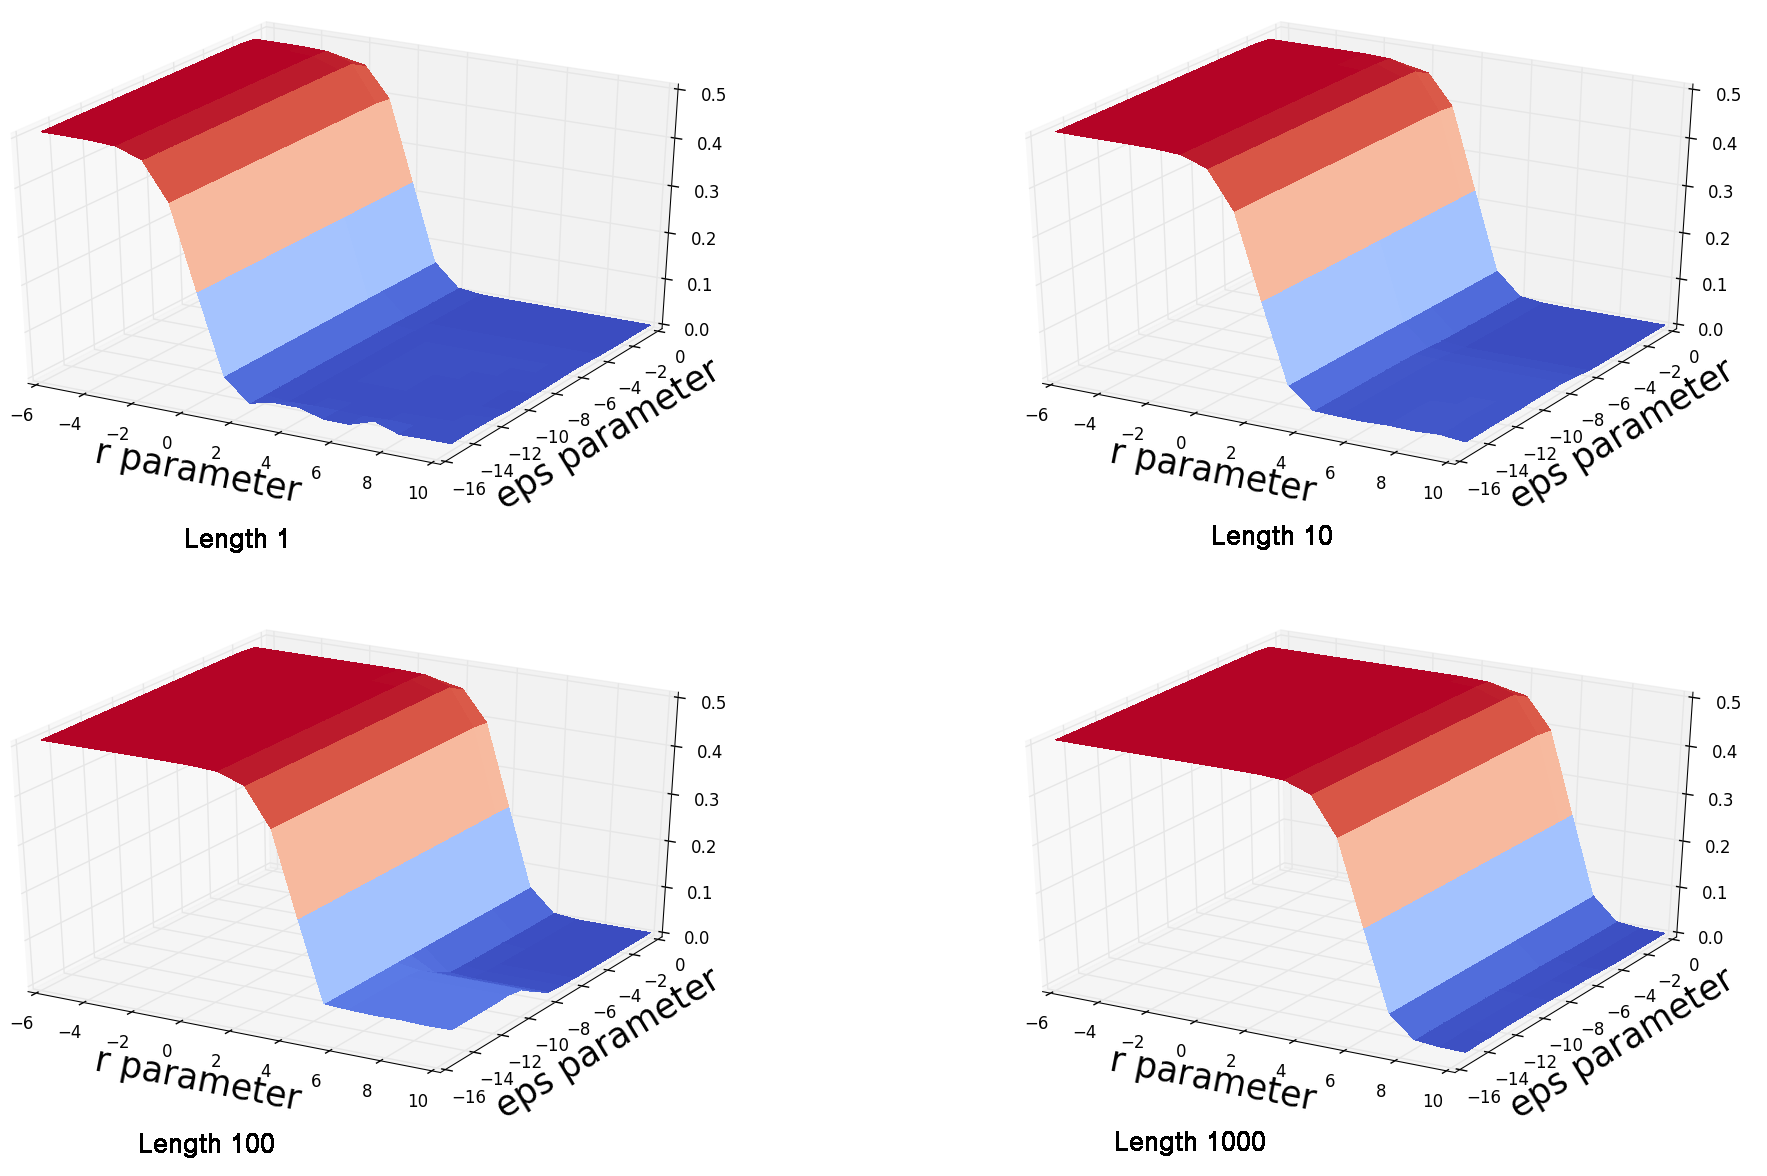
\includegraphics[width=1\textwidth]{figure_1.png}} \protect\caption{\label{fig14}Tuning data for the penalty method to find a scaling relationship between the size (upper left to lower right figure) of problem, penalty parameter and error - using logarithmic scales}
\end{figure} 

To find an optimum penalty parameter it is vital to base the calculation on random triangles limited to a fixed size boundary box. In order to maintain consistency in the randomness of the triangles, in addition to different sizes of boundary boxes, fixed length triangles are tested using random rotations. So it is guaranteed that triangles pair are always random in size and all possible cases are examined. For different scales of boundary boxes, it was interesting to find a linear relationship between the size of the boundary space, size of triangle and the penalty parameter. As it is shown in Figure \ref{fig14} for different sizes of triangles, the penalty parameters are linear with respect to the optimal equation that is derived based on the triangles size is: 
\begin{equation}
r_{optimal} = s*10^{(log10(s)+10)} 
\end{equation}

where s is the the size of the triangle boundary. The error is shown for a hundred thousand of pairs of triangles and it follows the optimal r penalty parameter. eps is the parameter for regularizing the Hessian matrix.


\begin{figure}[!h]
\centerline{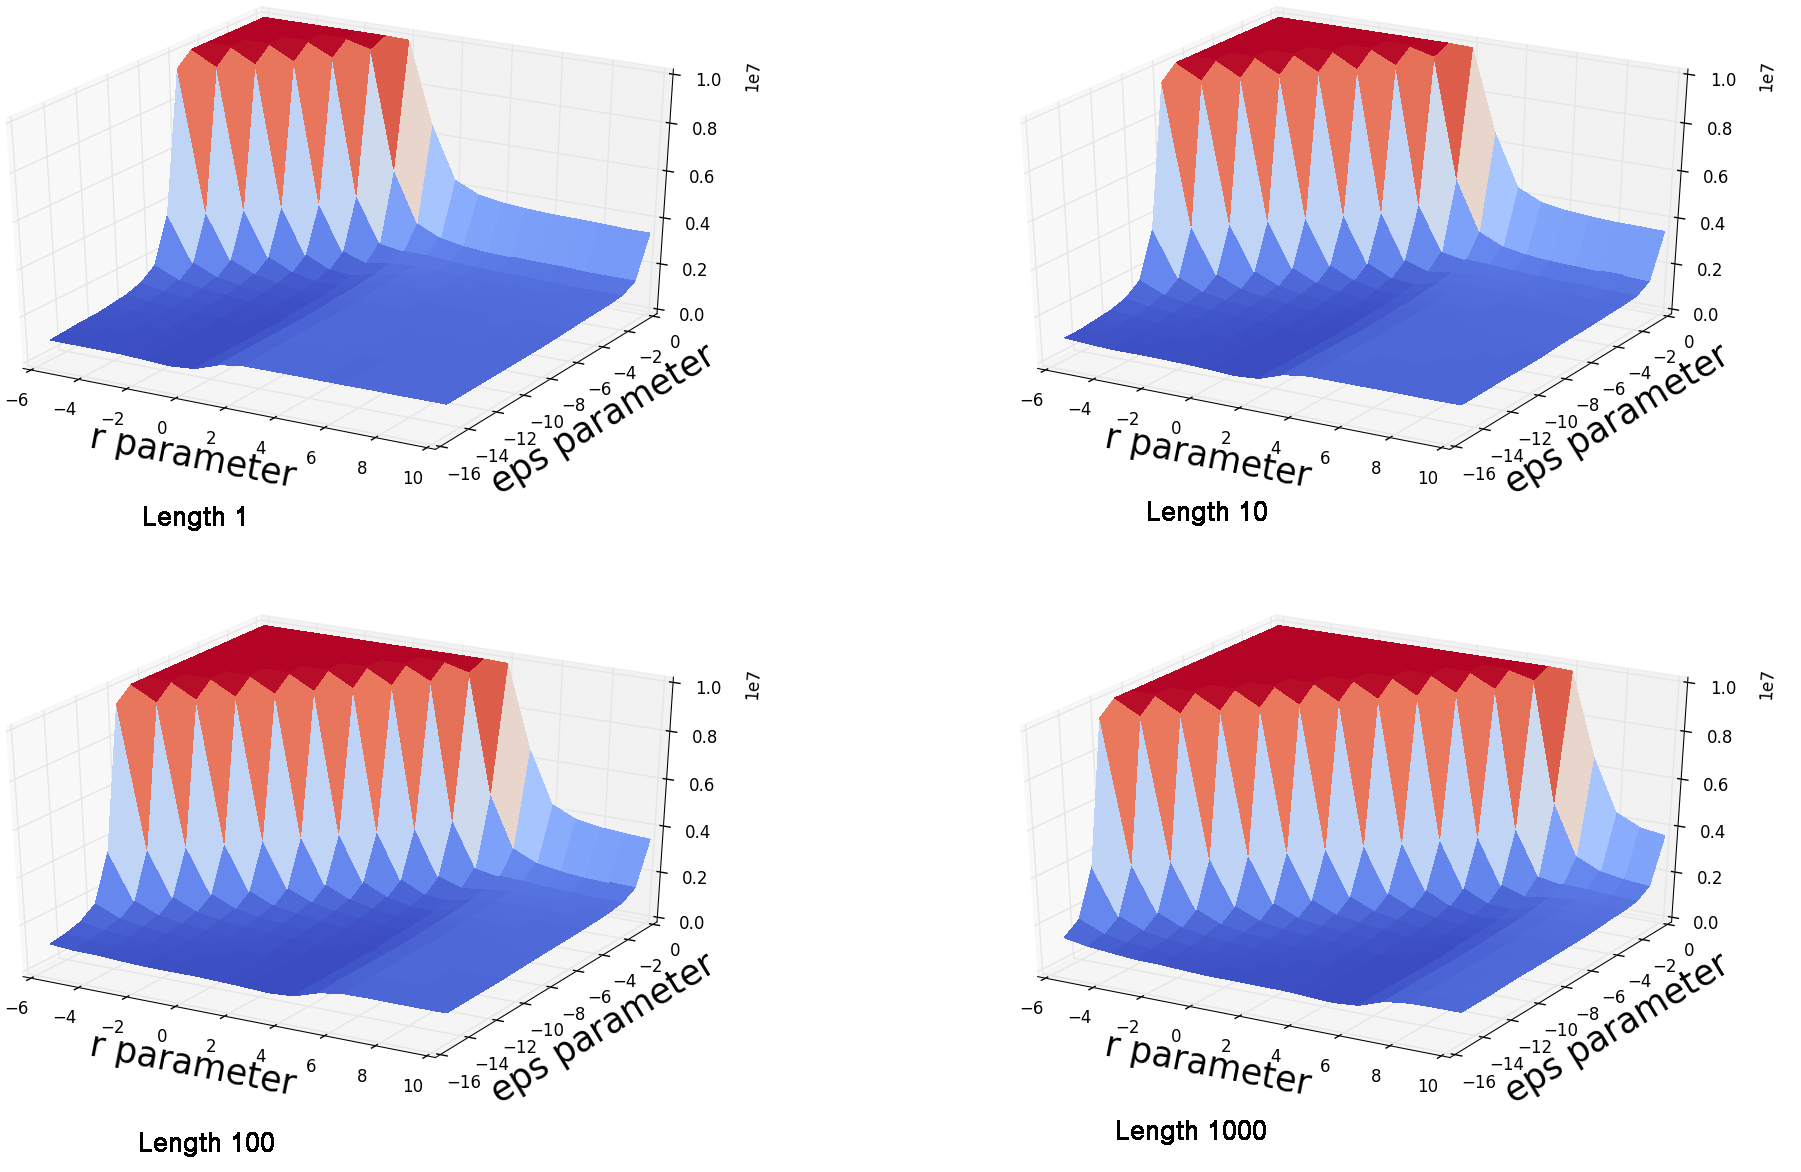
\includegraphics[width=1\textwidth]{figure_2.png}} \protect\caption{\label{fig15}Relationship between eps and number of iterations for different lengths of triangles. Optimal eps should be low and increased depending on the r parameter.}
\end{figure} 

The epsilon Hessian matrix regularization parameter has to be tuned based on the length of the triangles. It is necessary to see how epsilon behaves and how it is not only affecting the failure rate at specific sizes of triangles but also the number of Newton iterations. Tuning eps reveals that in order to achieve low number of Newton iterations at an average 3-4 iterations (~300,000 - 400,000 iterations average for 100,000 triangle pair calculation), eps has to be low for small triangles, We then linearly increase it as the size of triangles increases. But care has to be taken because there is a margin for achieving low optimal iterations when combined with the penalty tuned parameter. Having a very low epsilon parameter doesn't necessarily mean optimal iterations, eps is adjusted using a coefficient of boundary size.

Debugging and experiments on the prototype code in MATLAB show that the first and second Newton iterations oscillate around the convergence point, and the third converges to the solution(unless the point on the triangle is in the corner). The eps perturbation along the diagonal hessian can be increased at this point to complete the convergence since we know it is that area that should converge. This is tested and it works, the error is at the minimum at four iterations, with two points corresponding to the two triangles being correct. It should be noted that because penalty is used and because of the way it works mathematically (see penalty section), it is inevitable that the solution has to be in a position spatially outside (difference seen by the error values, see Figure \ref{fig14}). Epsilon initially cannot be too high but also not low because the solver cannot get the right direction (eps-r-iteration graph, Figure \ref{fig15}). The perturbation eps is increased after 3 steps for convergence with minimum error and minimum iterations. 

\begin{figure}[!h]
\centerline{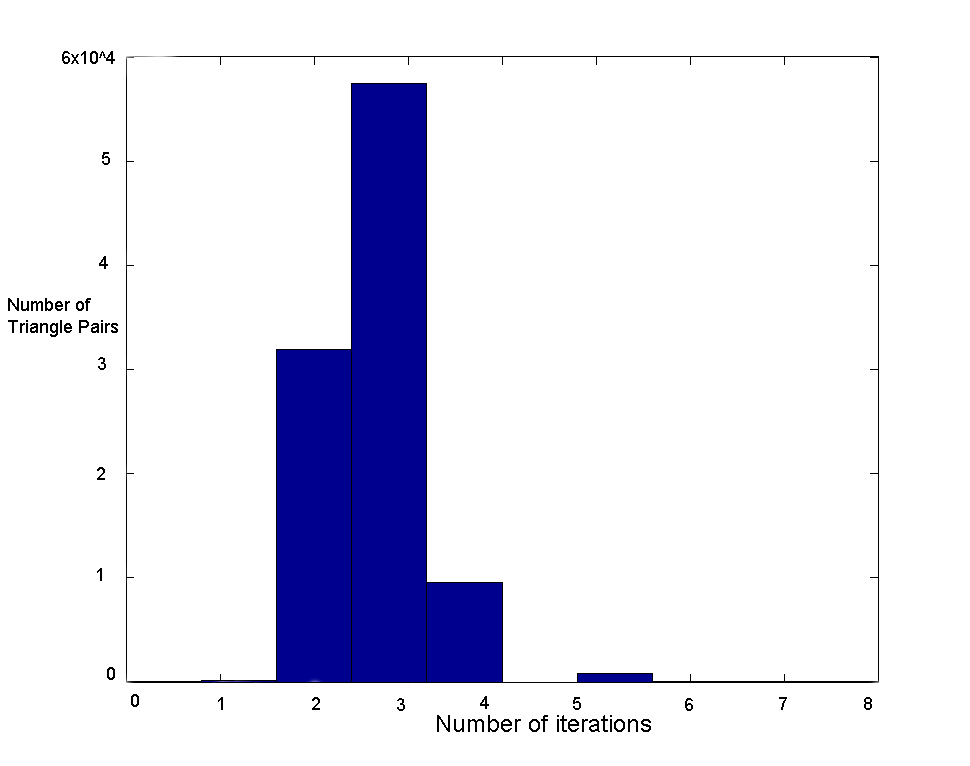
\includegraphics[width=0.8\textwidth]{norma.png}} \protect\caption{\label{fig16}Histogram that shows that most problems converge in three iterations}
\end{figure} 

\subsection{Remarks}

For both penalty and brute force methods, SIMD [39] version implementation required a significant amount of time of programming. Consider high performance programming techniques such as memory data alignment[24], data access , memory allocation, numerical computations and no redundant computations. We found that taking care of all the required compiler/hardware requirements caused significant speedups, many times program bugs are caused because of missing compiler pragma instructions for memory alignment. In addition, further slowdown may arise from non-vectorizable portions of the code. For example, the standard C library randomization function for the triangle coordinates had to switched with drand48() [41] Intel/GCC SIMD random function which is vectorized.

The revolutionary programming implementation involves the complete reconstruction of the serial algorithm to a parallel version with no aid of auto-vectorization compiler instruction. Our ISPC C code implementation of brute force and penalty methods shows this significant difference in code writing when compared their serial C versions. Re-arranging and thinking the structure of program at a low C language level is challenging because there is no easy way to apply formula to exploit data parallelism, and there is no easy to spot bugs in low level programming languages like C unless debugging and virtualization tool are used for profiling the execution of the code. So in practice, to develop robust code and avoid time in debugging human unreadable C parallel code, it is found that  segments of code has to be ported piece by piece from C serial to ISPC and tested at each stage.


\section{Performance Results}
All performance tests (Figure \ref{fig17}) used the latest AVX2 (Advanced Vector Extensions) instruction set on an Intel Sandy Bridge 2.0GHz i5 CPU with a memory of 600 MHz DDR3 RAM. For the barrier method isn't worth to do a performance comparison even though its C and ISPC version is implemented but not with great success due to its theoretical computational inefficiencies as discussed earlier in the report. Only the tuned penalty and brute force approaches are considered for real-world applications due their significant parallel speedup. The performance test comprises calculating the minimum distance between ten million pairs of triangles of length ten. The performance is scaled linearly for every magnitude length of pair triangle. 

\begin{figure}[!h]
\centering
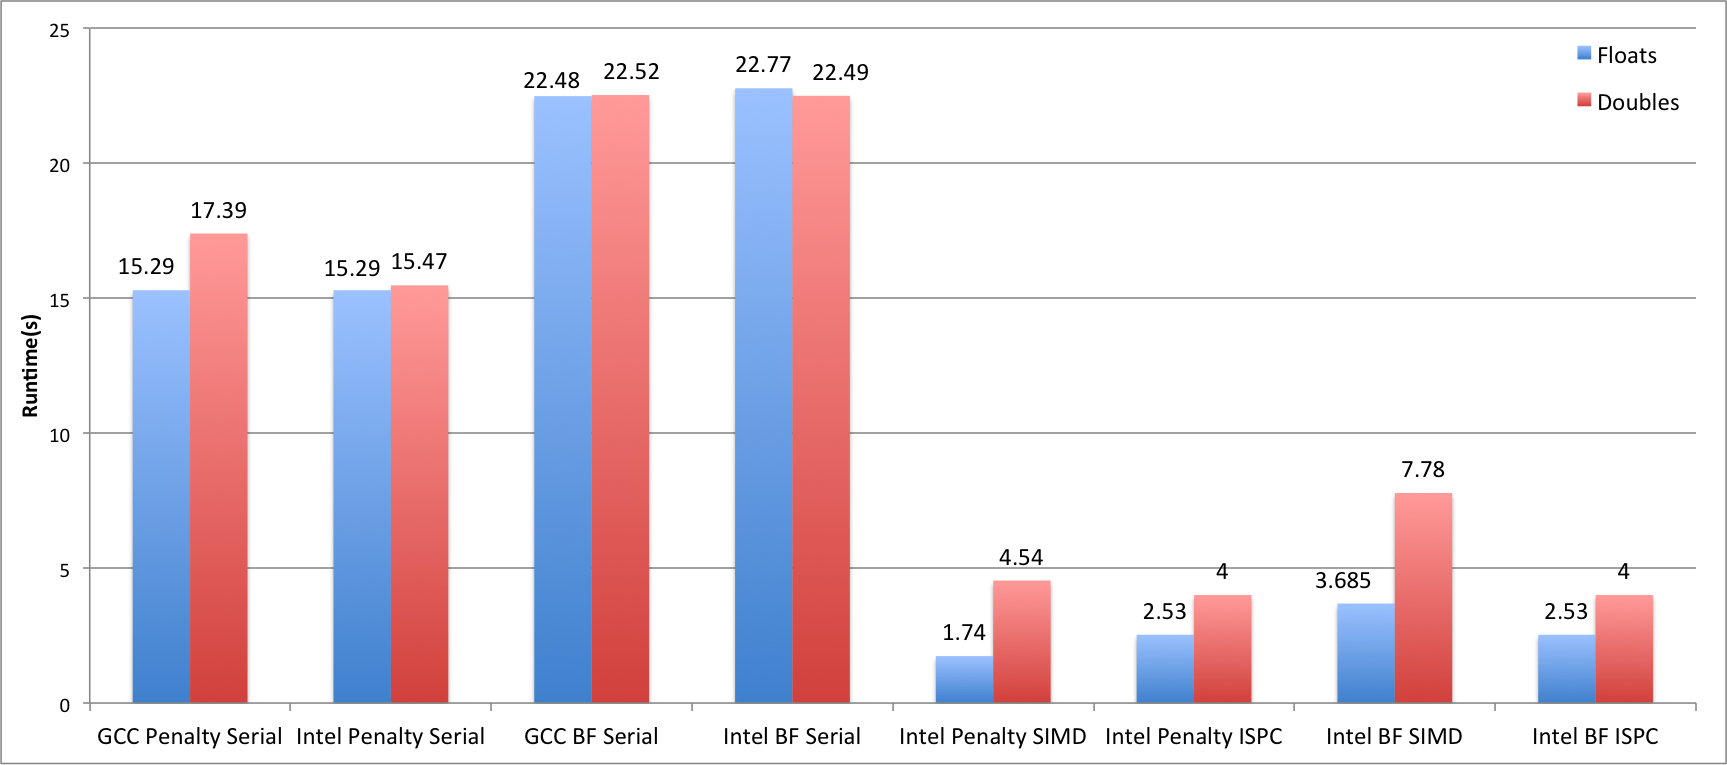
\includegraphics[width=1\textwidth]{perf} \protect\caption{\label{fig17}Run-time comparison of the sequential and parallel penalty and brute force methods using float and double precision, using ISPC, Intel, GCC compilers on a single AVX2 core.}
\end{figure} 

As it can be observed in Figure \ref{fig17}, the runtimes show that there is significant speedup when SIMD parallelism is used compared to sequential algorithm execution for all methods. For the brute force, serial Intel and GCC are the slowest with no significant difference in performance in using floats or double precision. That is due to little actual floating point computation. It has to be noted that our serial version is optimized considering memory bandwidth. For the Intel SIMD version of brute force, it can be seen that there is 6x speedup compared to its serial sequential variant using single precision. Speed up for double precision (~3x times), both results reflect the logical branching involved in brute force. Nevertheless the speed up is significant. The ISPC compiler for brute force is capable to do vectorization better for double precision than the Intel compiler, which makes the new vectorization compiler well-suited for SIMD programming. As we haven't studied the results assembles codes, we cannot identify where the difference between ISPC and C come from.

As penalty solver is an iterative method, its performance is dependent on the tuned parameters. The $r$ penalty parameter and $eps$ are calculated automatically based on the tuning and algorithm study performed. Moreover, the technique discussed in the implementation chapter for converging in 4 iterations is used without losing significant numerical precision. The penalty method reaches the physical limits of SIMD architectures with 4x speed up for double precision and 8x speedup for single precision. This makes it the fastest algorithm. Intel compiled serial code is significantly faster than Intel and GCC versions of Brute force. GCC compilers for serial are slightly slower, but still faster than brute force GCC serial. ISPC, Intel compiler for SIMD show that they are very fast, slightly showing a speedup for penalty over brute force. 

\begin{table}[h]
\begin{center}
    \begin{tabular}{ | l | l | l | p{5cm} |}
    \hline
\multicolumn{3}{ |c| }{Intel C++ Compiler Sequential Double Precision} \\
\hline
    Algorithm & Penalty Method & Brute Force Method\\ \hline
    Runtime unhalted (s) & 15.47 & 22.49  \\ \hline
    MFLOPS/s & 1073 & 962  \\ \hline
    CPI & 0.49 & 0.48 \\ \hline
    Memory BW M/s & 579 & 408 \\ \hline
    Data Volumn GB & 6.7 & 6.77 \\ \hline
    \end{tabular}
    \caption{64bit sequential computation; solving ten million random triangle pairs using the two methods.}
    \label{table1}
\end{center}
\end{table}

It can be observed see from performance measurements in Table \ref{table1} using likwid [49] that for serial double precision (same for single precision) both methods are not memory (Memory BW Bandwidth Megabyte per second) but compute-bound. For the machine used, the maximum memory throughput is 13 GB/s, so memory bandwidth is not used to the maximum. That is a result of careful programming, and as mentioned in the implementation section, due to the fact unnecessary memory operations are reduced extensively. The data volumn in Gigabytes is the same for both methods, since both methods use the same amount of input and output data. That is the triangle coordinates, P, Q point solution on the two triangles T1, T2 and the calculated distance which is derived from P and Q vectors. The penalty method is managing to executes faster than brute force because it execute slightly more floating point operations than the brute force (Mega Flops per second MFLOPS/s).

\begin{table}[h]
\begin{center}
    \begin{tabular}{ | l | l | l | p{5cm} |}
    \hline
\multicolumn{3}{ |c| }{Intel C++ Compiler SIMD Double Precision} \\
\hline
    Algorithm & Penalty Method & Brute Force Method\\ \hline
    Runtime unhalted (s) & 4.54 & 7.78  \\ \hline
    MFLOPS/s & 3202 & 2808  \\ \hline
    CPI & 1.26 & 0.91 \\ \hline
    Memory BW M/s & 1424 & 902 \\ \hline
    Data Volumn GB & 5.15 & 5.2 \\ \hline
    \end{tabular}
    \caption{64bit SIMD computation; solving ten million random triangle pairs using the two methods.}
    \label{table2}
\end{center} 
\end{table}

In Table \ref{table2} it can be seen that the SIMD implementation for both methods increase performance significantly. Their serial counterparts they both achieve more than 2x times speedup, with penalty achieving  3.40x speedup, and brute force 2.89x speedup. The theoretical maximum speedup that is possible to achieve is 4x times for 64bit precision using a 256bit wide register, and even more speedup for wider 512bit registers that are available on Xeon Phi processors. Using ISPC compilers however as shown in Figure \ref{fig17} double precision achieve 4x speedup. For 32bit precision the speedup using AVX 256bit wide instruction sets is near 8x times as it can be seen in Figure \ref{fig17}. 


\begin{figure}[!h]
\centering
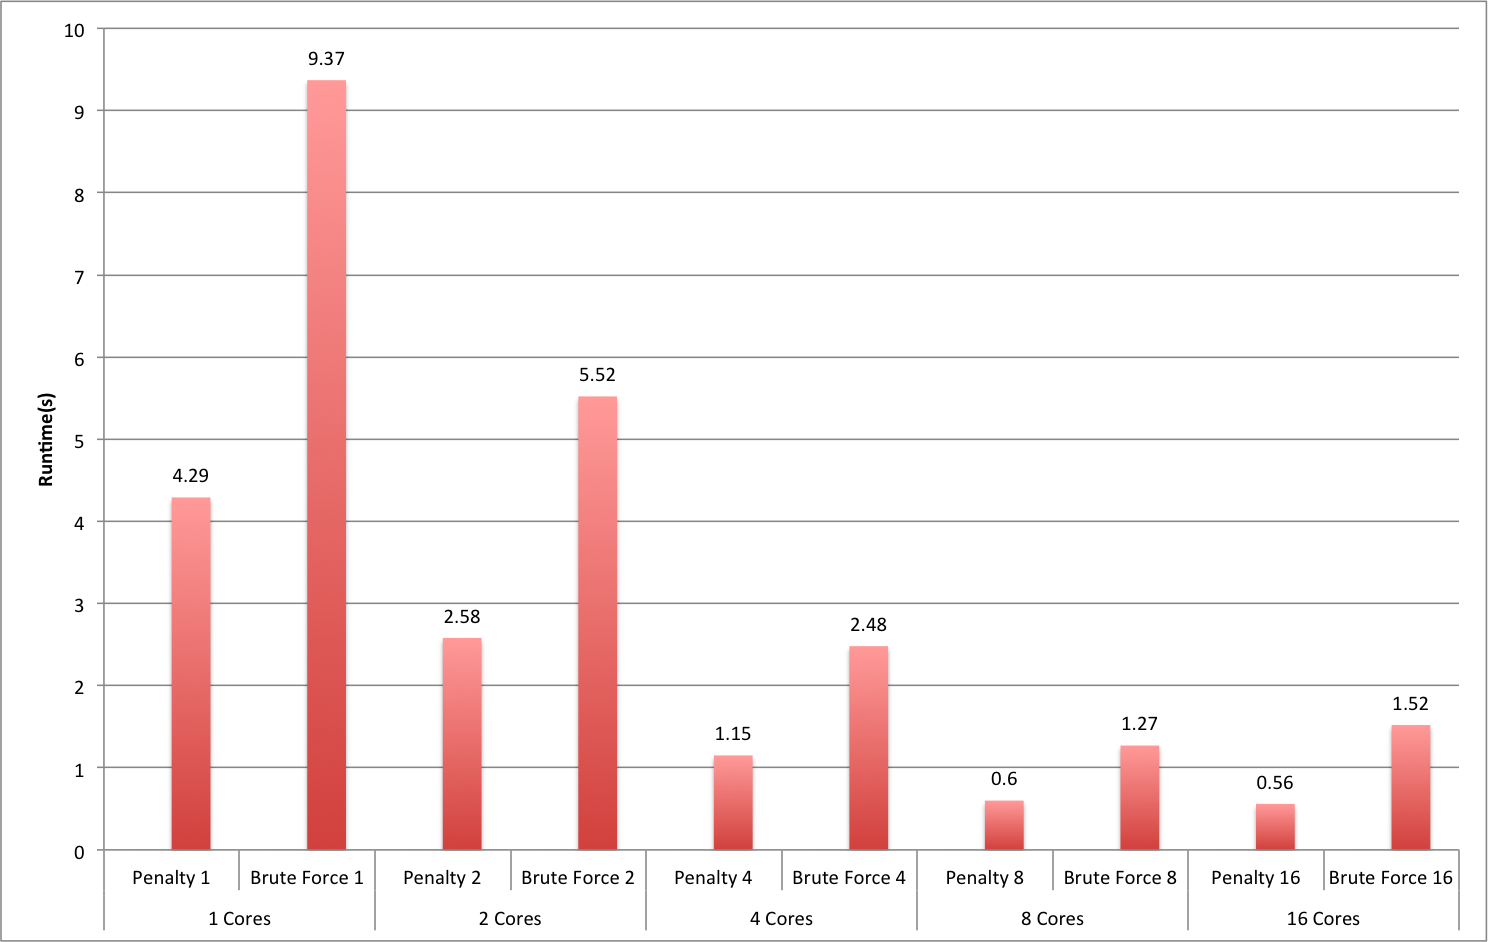
\includegraphics[width=1\textwidth]{openmp} \protect\caption{\label{fig18}Run time comparison of the penalty and brute force method using threads (OpenMP 4.0).}
\end{figure}

SIMD parallelism is running on each cores. Because of the availability of multi-cores, the test is performed on different sets of core to observe performance scaling. Using OpenMP 4.0 for task based parallelism, the algorithms are run on one,two,four,eight,sixteen cores respectively. The Figure \ref{fig18} shows the runtime for each solver. It can be observed that there is speedup for both penalty and brute force until eight core, that is because the next eight cores are on another CPU socket, and there is not significant performance gain because of the communication bandwidth between the two sockets.

These performance comparisons are the result of extensive low level programming and tuning of parameters to optimize the solvers. The effort of looking into compiler specific instructions and architecture specific programming has resulted into optimal codes for this triangle to triangle minimum calculation. In practice the SIMD speedups show that both penalty and brute force solvers are suitable but in terms of performance penalty is more favorable, while brute force benefits its numerical robustness. Overall because of the reduced errors and tuning through experiments and testing in addition to performance, the penalty method is the best method to use using either ISPC or Intel compilers and up to eight core concurrency.


\clearpage

\section{Future Work}
The research conducted until now involved study of algorithms in computational geometry, and it gives the required background knowledge for further research in the context of contact mechanics. Now a good robust algorithm for measuring the distance between triangles is implemented and it can be used as the building block in a Discrete Element Method (DEM) software package. There are few major aspects in this further work. Domain decomposition and data structures for storage of triangle information and load balancing of data structures for shared memory and distributed computation[19].

Load balancing is the next investigation for state of the art decomposition of space and subsequently the processing of parallel data in a distributed computing system (Message Passing Interface [7]) ). Incorporating the triangle distance algorithm on top of an optimal load balancing framework, provides the foundation for the development of a parallel particle simulation software for contact mechanics. The load balancing research involve multiple stages; firstly it is the decomposition of space into a well balanced in terms of computation and in terms of number of triangles on all compute nodes and on all processor cores. So far, the pairs just have been split naively without spatial context, then the parallel storage of the underlying particles and bodies/surfaces  are described. There are data structures that can store the partitioning of triangles space (k-d trees [25]). Sophisticated construction of radix trees can be used hierarchically or in parallel using space filling curve indexing [25]. Future work involve investigation and construction of such a load balancing data structure that is suitable for DEM codes. The next stage then is sorting of the data in parallel efficiently to redistribute and decompose again at every time step of the simulation. These are areas of research that are significant to investigate because to my knowledge there is no vectorized parallel Discrete Element code that include triangular elements for contact mechanics simulation. And I believe working with low level abstraction (no object oriented programming, low level programming) will create a significant high performance simulation software for large scale computing. 

With load balancing completed, my work will focus on the efficient implementation of contact mechanics Discrete Element Method [15,28] framework. As an application I will be performing the nuclear reactor contact simulation for Industry EDF, that requires this tool. In terms of contact mechanics, my research at this stage will involve the optimal SIMD implementation of codes that involve rigid kinematics and contact dynamics, considering fracturing as the last feature. The mechanics code will be studied primary from SOLFEC [27] as it includes an implicit contact solver, and is the closest thing to an open source real-world implementation of high performance contact mechanics.


\subsection{Work Packages}

WP 1. Load Balancing: Domain Decomposition
\begin{itemize}
\item Description: The work package will address the issue of decomposing the space of the triangles. Triangles are defined as points in space and computation/simulation is derived from these points. The decomposition has to be performed such that the computational workload is spread across all compute nodes or processors. The underlying data structure that will allow fast storage and decomposition of both bodies and triangles particles has to be investigated. SIMD vectorization of the decomposition algorithm will also be required.
\item Risk: none
\end{itemize}

\clearpage

WP 2. Load Balancing: Shared Memory Balancing 
\begin{itemize}
\item Description: Based on the domain decomposition performed in the previous work package, task based parallelism will be used to communicate data. The parallel multi-core algorithm will optimize the load balancing on one compute node. OpenMP 4.0 will be used extensively for share memory load balancing of the underlying triangles.
\item Risk: Dependency in work on domain decomposition. Availability of a shared memory compute node.
\end{itemize}

WP 3. Load Balancing: Distributed Memory Balancing 
\begin{itemize}
\item Description: Multi-node high performance computers is the primary computing architecture for DEM simulation. So research will involve implementation of load balancing the workload to a distributed computer. The developed algorithm will use the message passing interface (MPI) in combination with domain decomposition and shared memory computing as well as SIMD parallelism. The completion of this work will conclude the required high performance computational infrastructure to do DEM simulation, and for the computational mechanics to be build on top. 
\item Risk: Availability of message passing interface (MPI) enabled compute cluster. Hamilton HPC availability for measurement tests.
\end{itemize}

WP 4. DEM: Rigid Body Kinematics (parameterisation of rotation)
\begin{itemize}
\item Description: This work package will address the issue of parameterization of the body rigid rotation most suitable in the context of HPC computing and vectorization. The incremental rotational angle based representation in combination with the exponential map based update will be compared with the quaternion based representation from the point of view of their suitability and scalability in the SIMD setting.
\item Risk: none
\end{itemize}

WP 5. DEM: Rigid Body Dynamics (integration of rigid rotation)
\begin{itemize}
\item Description: This work package will address the issue of the integration of the equations of rigid body motion. Several time stepping techniques will be reviewed and a most suitable one, from the point of view of an efficient SIMD implementation, will be identified. Also, the way to formulate the dynamics in terms of the “total” or “updated” approach will be decided upon, looking from the perspective of the representation of rigid bodies as data (and data structures and dependencies between them) within an HPC DEM code.
\item Risk: none
\end{itemize}

WP 6. DEM: Shared Memory
\begin{itemize}
\item Description: A completely functional DEM code combining both intra-node (shared memory / SIMD) and inter-node (MPI distributed memory, possibly one-sided communication based) parallelism. This will build on the load balancing work packages as well as WP 4. and WP 5.. The triangle to triangle distance query developed during the first year of the studies will be incorporated as the core geometrical primitive driving the contact detection.
\item Risk: perhaps a lack availability of suitable HPC hardware to test the evolving implementation could be a hindrance.
\end{itemize}

WP 7. DEM: Fragmentation (Modeling of Fragmentation)
\begin{itemize}
\item Description: This is the final aspect of a general multi-rigid-body type simulator, that is practically needed from the point of view of the EDF energy application context. Fragmentation of graphite bricks during seismic events is a prominent aspect of risk and the ability to simulate it efficiently is therefore clear. Within this work package an efficient algorithmic way to geometrically represent and introduce fragmentation within a previously developed DEM framework will be devised. Also, the aspect of fragmentation criteria, from the mechanics points of view, as suitable in the rigid body context, will be addressed and applied.
\item Risk: necessity to incorporate large source code changes to handle fragmentation could be a risk; there this potential feature of the simulation which need to be incorporated into the software design at an earlier stage.
\end{itemize}

WP 8. DEM: Paraview Plugin;
\begin{itemize}
\item Paraview plugin; Viewing and storing large data sets base on moving rigid meshes, driven by rigid body motion, can be inefficient if positions of al triangles are stored for all time steps. It is much more effective to only store the initial positions followed by outputting the minimum representation of the rigid body motion for every time step (position, rotation). A plugin for Paraview will be developed in order to effectively work with such optimised representation.
\item Risk:potentially setting up a suitable compilation environment for Paraview could be trouble some; perhaps writing a plugin within this environment might not be trivial as well; a possible mitigation would be to investigate also other possible HPC post-processors, such as VisIt or OVITO in order to identify a most accessible solution; also, just outputting data in a standard VTK format will simply work and be sufficient for the completion of the research itself (although it will not be efficient);
\end{itemize}

\subsection{Conferences}

- Training - Performance Analysis Workshop (PRACE) -  Durham
\begin{itemize}
\item June 25 - 26
\item To get a better understanding of the code performance and to guide performance engineering, it is inevitable for computational scientists and engineers to conduct measurements and to study the performance in detail; in the best case prior to rewriting software or manual tuning. Performance analysis tools, a generalisation of the classic profiler, are the right tools to obtain this insight. However, they themselves require a decent level of understanding, experience and expertise to be used economically – which adds to the hardness and complexity of the underlying problem. This workshop is one event in a sequence of meetings where performance analysis tools are introduced, some hands-on training is done and existing mature source code is analysed. It focusses primarily on MPI, as a sibling course on shared memory and manycore architectures is given at EPCC earlier in the year.
\end{itemize}

\clearpage

- Training - Node-level Performance Engineering (PRACE) -  Stuttgart, Germany 
\begin{itemize}
\item July 6 - 7
\item This course teaches performance engineering approaches on the compute node level. "Performance engineering" as it is defined it is more than employing tools to identify hotspots and bottlenecks. It is about developing a thorough understanding of the interactions between software and hardware. This process must start at the core, socket, and node level, where the code gets executed that does the actual computational work. Once the architectural requirements of a code are understood and correlated with performance measurements, the potential benefit of optimizations can often be predicted. They introduce a "holistic" node-level performance engineering strategy, apply it to different algorithms from computational science, and also show how an awareness of the performance features of an application may lead to notable reductions in power consumption.
\end{itemize}

-Conference - SIAM Parallel Computing - Paris, France
\begin{itemize}
\item February 2016
\item Conference paper on current research on triangles with load balancing. Link: http://www.siam.org/meetings/pp14/
\end{itemize}

-Conference - Euro Par
\begin{itemize}
\item Autumn 2016
\item Conference paper on research on DEM with load balancing. Link: http://www.europar2015.org/
\end{itemize}

-Conference - International Supercomputing Conference
\begin{itemize}
\item May 2017
\item Whole Thesis/Project Research Paper. Link: http://www.isc-events.com/isc14/
\end{itemize}

\begin{sidewaysfigure}[!h]
\centering
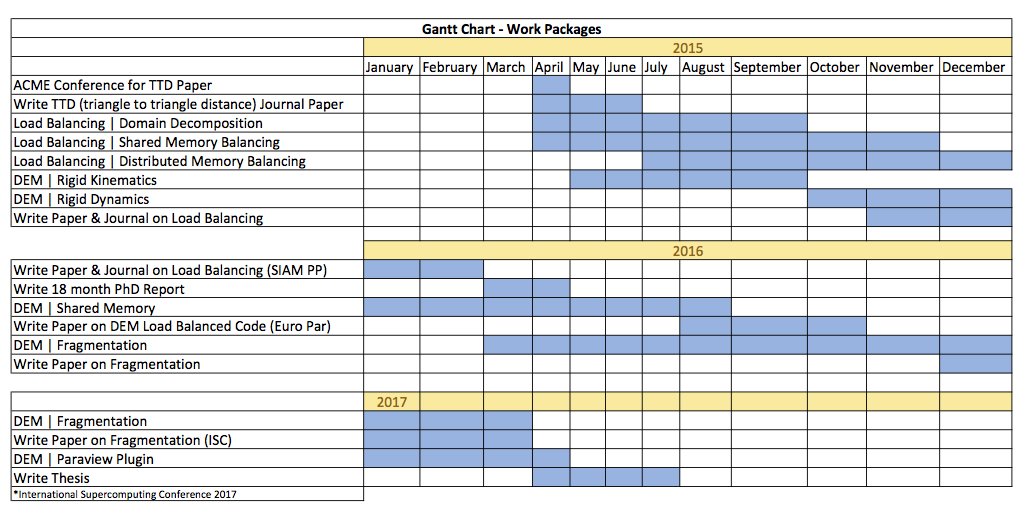
\includegraphics[width=1\textwidth]{chart} \protect\caption{\label{fig19}Timeline of Project}
\end{sidewaysfigure} 
\clearpage

\section{Appendix}
\subsection{Line Search}
There are times where it is not possible to have the derivatives to retrieve information about the curvature of the problem. For such cases there are available methods[8] for solving minimization problems without the requirement of using the derivatives of the objective function.
These type of algorithms, are often used as an enhancement step in the minimization process for methods that use Newton iterations. They are often used to enhance a Newton step depending on the specific problem as a numerical technique that determine the required step size for each of the Newton steps at each iteration for the global minimization problem. So depending on the line search algorithm there is a technique for determining the Newton step size, and it this is algorithm is acting independently to solve the sub-problem of minimizing the required Newton step. So for example let the step size be $\lambda_{k}$ then the iterative method is process such as $x_{k+1} = x_{k} + \lambda_{k} d_{k}$ where $x_{k}$ is a point and $d_{k}$ is the direction. The line search involve the minimization of the one dimensional sub-problem $f(x_{k} + \lambda d_{k})$. The minimization process for determining $\lambda$ involve the search of the ideal value for $\lambda$ over an interval $[a,b]$, this interval is called the interval of uncertainty and there are a couple of methods for solving the problem for $\lambda$ when there is a function $\theta$ such that it is defined in terms of function $f$ of several variables: $\theta(\lambda) = f(x + \lambda d)$.

To reduce the Newton steps when using the barrier method, various line search methods are investigated to assist the search to arrive to a solution. Line search methods included dichotomous search, golden section search, Fibonacci search. [8] The line search can be used for the penalty method but it is not adding any benefit solutions can converge fast (two, three iterations) and it would add an extra computational overhead. 
In the case of barrier method, line search safeguards the search from leaving the feasible region by doing smaller Newton Steps but then the performance is not adequate to the penalty anymore because of the additional line search code.

\subsubsection{Bisection Method}
The easiest to understand line search method is the bisection method. In the bisection search method the search for the minimum value for $\lambda$ over the interval of uncertainty can be said that is algorithmically similar to the dichotomous divide and conquer binary search algorithm. So for a constant value $e$ which is the tolerance for the search and $l$ the final length of the interval of uncertainty, the following pseudocode describes the search:  

\begin{algorithm}
\begin{lyxcode}
1.WHILE(1)

2.~~~~IF $(b_{k} - a_{k}) < l$

3.~~~~~~~~	BREAK

4.~~~~ELSE

5.~~~~	~~~~$\lambda_{k} = ((a_{k}+b_{k})/2) - e$

6.~~~~	~~~~$m_{k} = ((a_{k}+b_{k})/2) - e$		

7.~~~~~~~~IF $(\theta(\lambda_{k} < \theta(m_{k}))$

8.~~~~~~~~~~~~	$a_{k+1} = a_{k}$

9.~~~~~~~~~~~~	$b_{k+1} = m_{k}$
	
10.~~~~~~~~ELSE

11.~~~~~~~~	~~~~$a_{k+1} = \lambda_{k}$
	
12.~~~~~~~~~~~~	$b_{k+1} = b_{k}$

13.~~~~~~~~ENDIF

14.~~~~ENDIF

15.ENDWHILE

\end{lyxcode}
\protect\caption{\label{alg6}Bisection Line Search Method}
\end{algorithm}

The algorithm is operating on a interval $a, b$, in the interval there are the points $\lambda $ and $m$, that are $e$ away from each other. 
$a, b$ boundaries are updated and get the value of either $\lambda$ or $m$ and that defines the nature of bisecting the area based on iteratively testing the value of $\theta$. 


\subsubsection{Golden Section Method}
The golden section method [8] is a more efficient search scheme than bisection. The golden section search is characterized from the reduction rate when minimizing the function $\theta$, using the golden ration. The algorithm operates such that the length of the new interval of uncertainty $b_{k+1} - a_{k+1}$ does not depend upon the outcome of the kth iteration, that is whether $\theta (\lambda_{k}) > \theta (m_{k})$ or $\theta (\lambda_{k}) \leq \theta (m_{k})$. Therefore it must be such that $b_{k}-\lambda_{k} = m_{k} - a_{k}$. 

\begin{algorithm}
\begin{lyxcode}
1.WHILE(1)

2.~~~~IF $(b_{k} - a_{k}) < l$

3.~~~~~~~~~~~~BREAK

4.~~~~ELSEIF $(\theta(\lambda_{k} > \theta(m_{k}))$

5.~~~~~~~~~~~~$a_{k+1} = \lambda_{k}$

6.~~~~~~~~~~~~$b_{k+1} = b_{k}$

7.~~~~~~~~~~~~$\lambda_{k+1} = m_{k}$

8.~~~~~~~~~~~~$m_{k+1} = a_{k+1} a(b_{k+1} - a_{k+1})$

9.~~~~~~~~~~~~k = k+1	

10.~~~ELSEIF $(\theta(\lambda_{k} \leq \theta(m_{k}))$

11.~~~~~~~~~~~~$a_{k+1} = a_{k}$

12.~~~~~~~~~~~~$b_{k+1} = m_{k}$

13.~~~~~~~~~~~~$m_{k+1} = \lambda_{k}$

14.~~~~~~~~~~~~$\lambda_{k+1} = a_{k+1} + (1 - a)(b_{k+1} - a{k+1})$

15.~~~~~~~~~~~~$k = k+1$

16.~~~~ENDIF

17.ENDWHILE

\end{lyxcode}
\protect\caption{\label{alg7}Golden Section Line Search Method}
\end{algorithm}
\clearpage

\subsubsection{Fibonacci Method}

Similarly to the golden section method, the Fibonacci method [8] is using the Fibonacci sequence. The method in contrast to the golden ratio method is updating the length of the interval of uncertainty at every next iteration using the Fibonacci sequence. In addition  unlike the bisection or golden method, the Fibonacci search method requires that the total number of observation be specified beforehand. The length of the interval of uncertainty is reduced at iteration k by the factor $F_{n-1}/F_{n-k+1}$. Therefore n must be chosen such that it reflects the accuracy required.
\begin{algorithm}
\begin{lyxcode}
1.WHILE(1)

4.~~~~IF $(\theta(\lambda_{k} > \theta(m_{k}))$

5.~~~~~~~~$a_{k+1} = \lambda_{k}$

6.~~~~~~~~$b_{k+1} = b_{k}$

7.~~~~~~~~$\lambda_{k+1} = m_{k}$

8.~~~~~~~~$m_{k+1} = a_{k+1} + (F_{n-k-1}/F_{n-k})(b_{k+1} - a_{k+1})$

9.~~~~~~~~IF $(k == n-2)$

10.~~~~~~~~~~~~$\lambda_{n} = \lambda_{n-1}$
				
11.~~~~~~~~~~~~$m_{n} = \lambda_{n-1} + e$

12.~~~~~~~~~~~~IF $\theta (\lambda_{n}) > \theta (m_{n})$
					
13.~~~~~~~~~~~~~~~~$a_{n} = \lambda_{n}$
					
14.~~~~~~~~~~~~~~~~$b_{n} = b_{n-1}$ 

15.~~~~~~~~~~~~ELSE IF $\theta (\lambda_{n}) \leq \theta (m_{n})$
					
16.~~~~~~~~~~~~~~~~$a_{n} = a_{n-1}$
					
17.~~~~~~~~~~~~~~~~$b_{n} = \lambda_{n}$
					
18.~~~~~~~~~~~~ENDIF

19.~~~~~~~~~~~~BREAK

20.~~~~~~~ELSE 

21.~~~~~~~~~~~~$k = k+1$

22.~~~ELSEIF $(\theta(\lambda_{k} \leq \theta(m_{k}))$

23.~~~~~~~~$a_{k+1} = a_{k}$

24.~~~~~~~~$b_{k+1} = m_{k}$

25.~~~~~~~~$m_{k+1} = \lambda_{k}$

26.~~~~~~~~$\lambda_{k+1} = a_{k+1} + (F_{n-k-2}/F_{n-k})(b_{k+1} - a_{k+1})$

27.~~~~~~~~IF $(k == n-2)$

28.~~~~~~~~~~~~$\lambda_{n} = \lambda_{n-1}$
				
29.~~~~~~~~~~~~$m_{n} = \lambda_{n-1} + e$

30.~~~~~~~~~~~~IF $\theta (\lambda_{n}) > \theta (m_{n})$
					
31.~~~~~~~~~~~~~~~~$a_{n} = \lambda_{n}$
					
32.~~~~~~~~~~~~~~~~$b_{n} = b_{n-1}$ 

33.~~~~~~~~~~~~ELSE IF $\theta (\lambda_{n}) \leq \theta (m_{n})$
					
34.~~~~~~~~~~~~~~~~$a_{n} = a_{n-1}$
					
35.~~~~~~~~~~~~~~~~$b_{n} = \lambda_{n}$
					
36.~~~~~~~~~~~~ENDIF
				
37.~~~~~~~~~~~~BREAK

38.~~~~~~~~ELSE 

39.~~~~~~~~~~~~$k = k+1$

40.~~~ENDIF

41.ENDWHILE

\end{lyxcode}
\protect\caption{\label{alg8}Fibonacci Line Search Method}
\end{algorithm}

\clearpage


\begin{thebibliography}{99}


\bibitem{Mokhtar}
Mokhtar S. Bazaraa, Hanif D. Sherali, C. M. Shetty. Nonlinear Programming: theory and algorithms. John Wiley and Sons, Inc. 1993.

\bibitem{Ted}
Ted Belytschko, Wing Kam Liu, Brian Moran. Nonlinear Finite Elements for Continua and Structures. Wiley. 2000

\bibitem{William}
William Bittle. GJK (Gilbert Johnson Keerthi)Available at: \url{http://www.dyn4j.org/2010/04/gjk-gilbert-johnson-keerthi/}


\bibitem{Stephen}
Stephen Cameron. Computing the distance between objects. Available: http://www.cs.ox.ac.uk/people/stephen.cameron/distances. Oxford University. 2014

\bibitem{Todd}
Todd S. Coffey, C. T. Kelley, David E. Keyes. Pseudo-transient continuation and differential-algebraic equations. {\em SIAM J. Sci. Comp}, Vol. 25, 553--569. 2013.

\bibitem{Intel}
Intel Corporation. VTune(TM) Performance Analyzer for Linux. \url{https://software.intel.com/sites/default/files/m/6/5/2/c/f/6734-vtune_getting_started_linux.pdf} 2014. 

\bibitem{Jack Dongarra}
Jack Dongarra., Pete Beckman. The International Exascale Software Project roadmap. International Journal of High Performance Computing Applications. 3-60. Volume 25 Issue 1, February 2011.

\bibitem{David}
David Eberly. Intersections of a Set of Segments. Geometric Tools. Available at: \url{http://geomalgorithms.com/a09-_intersect-3.html}. 2008

\bibitem{David}
David Eberly. Intersection of Rays and Triangles. Geometric Tools. Available at: \url{http://geomalgorithms.com/a06-_intersect-2.html} 2008

\bibitem{David}
David Eberly. Planes and Distance of a Point to a Plane. Geometric Tools. Available at: \url{http://geomalgorithms.com/a04-_planes.html} 2008.

\bibitem{David}
David Eberly. Distance Between Point and Triangle in 3D. Geometric Tools. 2008

\bibitem{Christer}
Christer Ericson. Real-Time Collision Detection. Elsevier. 2005

\bibitem{Christer}
Christer Ericson. The Gilbert-Johnson-Keerthi algorithm. Elsevier. 2005

\bibitem{Gwendolyn}
Gwendolyn Fischer. Distance between a point and a triangle in 3D. Available at: \url{http://uk.mathworks.com/matlabcentral/fileexchange/22857-distance-between-a-point-and-a-triangle-in-3d}. MATLAB CENTRAL. 2009

\bibitem{Evghenii}
Evghenii Gaburova, Yuri Cavecchi. Xeon Phi Meets Astrophysical Fluid Dynamics. PRACE. 2014

\bibitem{George}
P.L. George, H. Borouchaki. Construction of tetrahedral meshes of degree two. International journal for numerical methods in engineering. 90:1156-1182. 2012.

\bibitem{GTS}
GTS. The GTS (GNU Triangulated Surface) Library. Available at: \url{http://gts.sourceforge.net/gallery.html} 2015.

\bibitem{Pedro}
Pedro Gonnet. Efficient and Scalable Algorithms for Smoothed Particle Hydrodynamics on Hybrid Shared/Distributed-Memory Architectures. SIAM Journal on Scientific Computing. 2014

\bibitem{John}
J. Harrison. Formal Verification of IA-64 Division Algorithms. Lecture Notes in Computer Science, pp. 233-251, Springer, 2000.

\bibitem{Hansen}
P. C. Hansen. The L-curve and its use in the numerical treatment of inverse problems. Computational Inverse Problems in Electrocardiology. 119-142. 2001.

\bibitem{Kris}
Kris Hauser. Robust Contact Generation for Robot
Simulation with Unstructured Meshes. {\em Intl. Symposium on Robotics Research}, 2013.

\bibitem{kris}
Kris Hauser. Locomotion and Manipulation Planning Toolkit. Available: https://github.com/krishauser/Klampt. GITHUB. 2011


\bibitem{Hughes}
T.J.R. Hughes, J.A. Cottrell, Y. Bazilevs. Isogeometric analysis: CAD, finite elements, NURBS, exact geometry and mesh refinement. Elsevier. 2004

\bibitem{Jim Jeffers}
Jim Jeffers, James Reinders. Intel Xeon Phi Coprocessor High-Performance Programming. Elsevier. 2013.

\bibitem{Tero}
Tero Karras. Maximizing Parallelism in the Construction of BVHs, Octrees and k-d Trees. High Performance Graphics. 2012

\bibitem{Koziara}
Koziara, T., Bićanić, N. A distributed memory parallel multibody Contact Dynamics code. International Journal for Numerical Methods in Engineering 87(1-5): 437-456. 2011.

\bibitem{Koziara}
Koziara, T. Computational Contact Dynamics. Available: https://code.google.com/p/solfec/. Google Code. 2014

\bibitem{Koziara}
Koziara, T. Particulate Media Simulator. Available: https://github.com/tkoziara/parmes. GITHUB. 2014

\bibitem{Sandia}
Sandia Lab. Hilbert curve for load balancing. Available at: \url{http://www.cs.sandia.gov/Zoltan/dev_html/dev_hsfc.html}. 2014

\bibitem{lazard}
Lazard. Intersection between a Line Segment and a Triangle. Available at: \url{http://www.loria.fr/~lazard/ARC-Visi3D/Pant-project/files/Line_Segment_Triangle.html}

\bibitem{Shin}
Shin-Jae Lee, Minsoo Jeon, and Dongseung Kim. Partitioned Parallel Radix Sort. Journal of Parallel and Distributed Computing 62, 656–668. 2002.

\bibitem{Shuo}
Shuo Li, Brian Rea, Jim Cownie. Extending Parallelism from Intel Xeon Processor to Intel Xeon Phi Coprocessor: A Structured, Stepwise Approach to Manycore Programming. Intel Corporation. 2014


\bibitem{Scherzer}
O. Scherzer Linz. The Use of Morozov's Discrepancy Principle for Tikhonov Regularization for Solving Nonlinear Ill-Posed Problems. Springer-Verlag. Computing 51, 45-60. 1993.

\bibitem{Tim}
Tim Mattson. A “Hands-on” Introduction to OpenMP. Intel Corp. 2014

\bibitem{nancy}
Nancy M., Amato Ravishankar, Iyer Sharad Sundaresan. A Comparison of Parallel Sorting Algorithms on Different Architectures. 1996.


\bibitem{Jorge}
Jorge Nocedal, Andreas Wächter†, Richard A. Waltz. Adaptive Barrier Update Strategies for Nonlinear Interior Methods. SIAM Journal on Optimization 19 (4) , 1674-1693. 2009.

\bibitem{OpenMP}
OpenMP. The OpenMP API specification for parallel programming. Available at: \url{https://software.intel.com/en-us/articles/32-openmp-traps-for-c-developers/} 2015.

\bibitem{Sergei}
Sergei Pereverzev, Eberhard Schock. Morozov's discrepancy principle for Tikhonov regularization of ill-posed problems in finite-dimensional subspaces. Numer. Funct. Anal. Optim., 21, 901-916. 2000.

\bibitem{Matt}
Matt Pharr, William R. Mark. ispc: A SPMD Compiler for High-Performance CPU Programming. Intel Corporation. Innovative Parallel Computing (InPar), 1 - 13. 2012. 

\bibitem{Khaled}
Khaled Rasheed. An Adaptive Penalty Approach for Constrained Genetic-Algorithm Optimization. Proceedings of the Third Annual Genetic Programming Conference. Morgan Kaufmann Publishers. 1998.

\bibitem{James}
James Reinders. High Performance Parallelism Pearls: Multicore and Many-core Programming Approaches. 2014

\bibitem{Samuel}
Samuel Hans Martin Roth. Bernstein-Bezier Representations for facial Surgery Simulation. Swiss Federal Institute of Technology. 2002.

\bibitem{Andrzej}
Andrzej Ruszczynski. Nonlinear Optimization. Princeton University Press. 2006

\bibitem{Nadathur}
Nadathur Satish, Mark Harris, Michael Garland. Designing Efficient Sorting Algorithms for Manycore GPUs. Parallel and Distributed Processing. 2009

\bibitem{Smith}
Alice E. Smith and David W. Coit. Constraint-Handling Techniques - Penalty Functions. Handbook of Evolutionary Computation, Institute of Physics Publishing and Oxford University Press, Chapter C5.2. 1997.

\bibitem{Dan}
Dan Sunday. Planes and Distance of a Point to a Plane Available: http://geomalgorithms.com. Geomalgorithms. 2014

\bibitem{Dan}
Dan Sunday. Distance between 3D lines and segments. Available: http://geomalgorithms.com. Geomalgorithms. 2014

\bibitem{Oren}
Oren Tropp, Ayellet Tal and Lian Shimshoni. A fast triangle to triangle intersection test for collision detection. Wiley. 2005

\bibitem{likwid}
J. Treibig. Likwid - Lightweight Performance Tools. 9th VI-HPS Tuning Workshop. University Versailles. Available: https://code.google.com/p/likwid/

\end{thebibliography}
\end{document}







